\documentclass[final,numrefs,twoadvisors,sort&compress,noinfo]{nddiss2e}
%\usepackage{amsmath}
%\usepackage{caption}
%\usepackage{color}
%\usepackage{float}
%\usepackage{fullpage}
%\usepackage{graphicx}
%\usepackage{longtable}
%\usepackage{multirow}
%\usepackage[nottoc]{tocbibind}
\usepackage{subcaption}
\usepackage{url}
\usepackage{epigraph}
\renewcommand{\textflush}{flushepinormal}
\setlength{\epigraphwidth}{0.7\paperwidth}
%\setlength{\pdfpagewidth}{\paperwidth}
%\setlength{\pdfpageheight}{\paperheight}
%\setcounter{tocdepth}{0}

%\renewcommand{\captionfont}{\small}

\newcommand{\degrees}{$^{\circ}$ \,}
\newcommand{\tablenote}[1]{\footnotesize NOTE: #1}
% \newcommand{\question}[1]{\textbf{#1}}

\begin{document}
\frontmatter

\title{REPLACING DOMAIN-SPECIFIC METHODS IN BIOINFORMATICS WITH MACHINE LEARNING TECHNIQUES}

\author{Ronald J. Nowling}

\work{Dissertation}

\degaward{Doctor of Philosophy}

\advisor{Scott Emrich}
\secondadvisor{Mary Ann McDowell}

\department{Computer Science and Engineering}

\maketitle

\makecopyright

\begin{abstract}
  Put an abstract here.
\end{abstract}


\tableofcontents
\listoffigures
\listoftables

\begin{acknowledge}
  \epigraph{\textit{Where one alone may be overcome, two together can resist. A three-ply cord is not easily broken.}}{Ecclesiastes 4:12, New American Bible (Revised Edition)}

  During the journey towards earning my Ph.D., I learned that a Ph.D. is not the work of one person alone but rather requires the support of an entire community. I am incredibly grateful and appreciative of the support that many have provided, both directly in helping me successfully complete my Ph.D. and helping me along the path towards a Ph.D. in the first place.

  First, I want to thank my family.  My grandmother Dr. Mary Ellen Jacobs, who earned her Ph.D. later in life after a successful first career as a musician, has always encouraged my intellectual pursuits, inspired me to pursue a Ph.D., opened doors to a position at UConn that started my research career, and provided an empthatic ear as someone who has walked the Ph.D. path before me.  My mother Erika Tracy has always enthusiastically supported (and helped finance!) my educational and scholarly pursuits -- I will be forever grateful of her embrace of my work and trust in my ability to set my own path. My grandfather James Jacobs was always ready with sound advice on people and character, which helped me grow as a person.  My fianc\'{e}e Marissa McCabe has stood by my side and been incredibly flexible while I've been working full time and working on my Ph.D. part-time over the last two years.

  I am incredibly grateful to my advisors, Profs. Mary Ann McDowell and Scott Emrich. Mary Ann  has served as an empaphetic mentor and reliable sounding board from my first day at Notre Dame.  When I decided to take a full-time position at Red Hat, Mary Ann immediately offered, without reservation, to take me on as her student so I could finish my Ph.D. and led a coordinated effort of professors in the Computer Science \& Engineering and Biological Sciences departments to work out the details.   Prof. Scott Emrich was incredibly kind to take me on as a late-stage Ph.D. student who was ``rebooting'' his Ph.D. topic while starting a full-time career.  Scott's mentoring has led me to finding tractable problems and establish a new research direction for myself.  Both took a risk when taking me on as a part-time student and placed a significant amount of trust in me.  Thank you to you both for helping me get to my defense.

  I'd like to thank my colleagues.  Jenica L. Abrudan has been a close friend and collaborator throughout my Ph.D.  I am grateful for the great deal of time she has spent patiently explaining biological concepts, offering constructive feedback, encouragement, and support, and being an awesome friend.  I could not have completed my Ph.D. without the support and encouragement of my management team and colleages at Red Hat.  I would like to thank Scott McClellan and Matthew Farrellee for their support and flexibility.  I would particularly like to thank Will Benton and Erik Erlandson for being open to discussing my ideas and offering constructive feedback, their help in improving my presentation skills, and advice on the overall Ph.D. process.

  I'd made quite a few friends during my time at Notre Dame, both inside and outside of the university.  Thank you to Badi' Abdul-Wahid, Kevin Kastner, Haoyun Feng, Yong Hwan Kim, James Sweet, Li Feng, Mallory Smith, Melinda Varga, and Reid Johnson for their friendship and sharing in the crazy ride that is grad school with me.  Bernardo, Theresa, and Ian Contreras opened their home to me, giving me family away from home. I'd like to thank Sironaj Hindawi, Alexa Robertson, and the larger Baha'i Michiana-area community; my friendships and time spent volunteering with them contributed to my overall development as a person.

  My journey to a Ph.D. started before Notre Dame, and I have many people to thank for helping me get here.  Thank you to profs. Larry Klobutcher, Michael Gryk, and Marty Schiller of the University of Connecticut Health Center for offering me summer research opportunities as a high and college student.  Jay Vyas, a Ph.D. student at the University of Connecticut Health Center, mentored me, helping me to grow in my technical skills, and has become a life-long friend; I am also grateful to Jay for referring me to Red Hat and opening those doors for me.  Thank you to Profs. Holger Mauch, Kelly Debure, and Trevor Cickovski from Eckerd College for the amount of time spent mentoring me and providing opportunities above and beyond the already strong undergraduate education they gave me.

  Last but not least, I would like to thank my committee: Profs. Kevin Bowyer, Greg Madey, Trevor Cickovski, and Zain Syed.  I appreciate the time and effort you've spent to guide me towards finishing my Ph.D.
  
\end{acknowledge}


\mainmatter


\chapter{Introduction}

Arthropod vectors are increasingly becoming important in emerging human disease outbreaks.  In addition to the recent Zika outbreak vectored by the mosquito \emph{Aedes aegypti}, linked to serious medical outcomes, nearly half of the world's population is still at risk of contracting malaria.  In 2015, 214 million malaria infections, resulting in 438,000 deaths, were reported. Nearly 90\% of the reported infections and deaths have occurred in Sub-Saharan Africa.  Mosquitoes in the \emph{Anopheles} genus are the sole vectors of the malaria-causing \emph{Plasmodium} parasites \cite{Neafsey2015,Neafsey2010,Lawniczak2010}. As such, efforts to control populations of insect vectors such as \emph{Anopheles gambiae} are key to efforts to eradicate malaria and other insect-borne diseases \cite{Holt2002}.

\emph{Anopheles} species have been subject to evolutionary adapations due to host-parasite interactions and specializations needed to thrive when living among and feed on humans \cite{Neafsey2015}. Population control efforts are informed through studies of insect biology and characterizerations of these adaptations, which are enabled by sequencing and comparative analysis of insect genomes.   Such studies have been fruitful, with results including the identification of chemosensory receptors responsible for detection of human hosts \textcolor{red}{CITE} and the molecular bases of variations in insecticide resistance between populations and species \cite{Lawniczak2010}.

Bioinformatic analysis of insect genomes is complicated by unique characteristics of insect biology.  For example, mammalian chemosensory receptors are G Protein Coupled Receptors (GPCRs), while insect chemosensory receptors are ion channels which are poorly-conserved on the sequence level.  Insect genomes tend to have low linkage disequilibrium (LD), or correlation  between variations located nearby on chromosomes, resulting in low statistical power when identifying interesting variations.

The larger bioinformatics community is adept at developing algorithms and accompanying software to meet such challenges.  However, constantly developing new tools is inefficient and can inhibit research progress.  Method development is time consuming and requires significant resources.

Development time and the number of bugs can be reduced through writing \emph{less new code} and and making more extensive usage of existing libraries. The machine learning community has invested significant effort into developing and standardizing around libraries for a variety of languages and platforms.  Libraries such as scikit-learn \cite{scikit-learn} have large users bases and have gained the respect of the scientific community for their quality, performance, active community of developers, and maturity. New algorithms are implemented reasonably quickly, releases occur on a regular schedule, and users can expect continued support.  Some of these libraries \textcolor{red}{CITE} are able to utilize GPUs and distributed computing to scale to massive data volumes.

\section{Contributions}
The key challenge is to demonstrate that standard machine learning techniques can be adapted to overcome the challenges facing bioinformatic analysis of insect vector genomes in place of more specialized methods.  In this dissertation, we demonstrate the role of machine learning methods in insect bioinformatics. 

We begin by analyzing the genomes and RNASeq expression of genes from two sand fly species, \emph{Lutzomyia longipalpis} and \emph{Phlebotomus papatasi}, which are vectors of leishmaniasis. \textcolor{red}{more details on results} These analyses provide background into the types of questions that biologists seek to answer and the challenges associated with insect genome bioinformatics.

Secondly, we describe a novel ensemble approach for identifying G Protein-Coupled Receptors (GPCRs) in insect vector genomes.  Existing GPCR classifiers such as GPCRHMM and PredCouple present several limitations: (1) they are trained using GPCRs from a diverse set of organisms including human (\emph{Homo homo sapiens}) and the fruit fly\emph{Drosophila melanogaster}, resulting in sub-optimal performance when applied to insect vectors and (2) their resulting scores can be difficult to interpret.  We describe a novel pipeline, called Ensemble*, that utilizes GPCRHMM and Pfam GPCR Hidden Markov Models (HMMs) but improves sensitivity, accuracy, and interpretability over GPCRHMM and Pfam HMMs alone. For each classifier, Ensemble* uses an empirical conditional probability function, trained on known GPCRs from the mosquitoes \emph{Aedes aegypti}, \emph{Anopheles gambiae}, the louse \emph {Pediculus humanus}, the honey bee \emph{Apis mellifera}, \emph{Drosophila melanogaster}, and \emph{Homo homo sapiens}, to estimate the probability that a protein is a GPCR given a score from the classifier.  An ensemble was formed from the classifiers by using a weighted average the classifiers' likelihood functions.  We evaluated the sensitivity and accuracy of Ensemble*, demonstrating improved sensitivities of up to 10\% on \emph{Aedes aegypti}, \emph{Anopheles gambiae}, \emph{Apis mellifera}, and \emph{Pediculus humanus} with no loss of sensitivity for \emph{Drosophila melanogaster} and \emph{Homo homo sapiens}. Using Ensemble*, we re-analyzed the GPCR repoirteres of the vectors \emph{Aedes aegypti}, \emph{Anopheles gambiae}, resulting in the identification of 30 additional putative GPCRs, of which 19 were validated and confirmed via sequence similarity to known GPCRs with BLAST.

Lastly, we describe a workflow for ranking SNPs from incipient \emph{Anopheles} species using Random Forests.  Along the way, we demonstrate the presence of bias using numerical experiments and describe appropriate solutions that can be used with standard, \emph{unmodified} implementations of decision trees available in popular machine learning libraries. We provide a software package called Asaph that implements the workflow using Python, numpy, scipy, and scikit-learn.  Asaph is applied to SNPs from \emph{Anopheles gambiae}, \emph{Anopheles coluzzii}, and two forms of \emph{Anopeheles funestus}, Folonzo and Kiribina, resulting in the identification of SNPs in genes previously reportedly to be associated with differences in insecticide resistance between the populations.

\textcolor{red}{sand flies -$>$ challenges in insect bioinformatics}

\textcolor{red}{ensemble* -$>$ existing bioinformatics tools can be adapted and improved for use on insect genomes by employing techniques from machine learning (ensembles) and statistics (conditional probabilities)}

\textcolor{red}{Asaph -$>$ more common machine learning techniques (e.g., Random Forests) can be used to replace more specialized bioinformatics techniques, allowing for the use of existing libraries and their advantages}

\textcolor{red}{draw conclusion, bringing argument back to original goal}

\section{Synopsis}
The rest of this dissertation is organized as follows:

\begin{itemize}
\item Chapter 2: Comparative analysis of the genomes of and RNASeq expression of genes from two sand fly species, \emph{L. longipalpis} and \emph{P. papatasi}.
\item Chapter 3: Evaluation of Hidden Markov Model (HMM)-based tools for identifying G Protein-Coupled Receptors (GPCRs) in insect vector genomes and demonstratation of how a simple approach for creating an ensemble of existing classifiers can improve accuracy by at least 5-11\%.
\item Chapter 4: Application of Random Forests to ranking SNPs from incipient species of \emph{Anopheles} mosquitoes.  We identify multiple sources of bias that can arise and provide solutions that utilize ``out-of-the-box'' implementations of decision trees.  We provide a software implementation of our workflow using the popular machine learning library sci-kit learn, which we apply to the study of SNPs from several \emph{Anopheles} species.
\end{itemize}

We conclude by identifying topics for further investigation. \textcolor{red}{expand}

\chapter{Comparative Genomic Analysis of \emph{P. papatasi} and \emph{L. longipalpis} Sand Fly Genomes}

\section{Introduction}
Leishmaniasis is a disease caused by protozoan parasites. Leishmaniasis occurs in multiple forms. Cutaneous leishmaniasis infects the skin, causing painful sores which can reoccur up to 20 years after infection, even in individuals who have been adequately treated. The deadly form visceral leishmaniasis is the second-largest parasitic killer in the world, responsible for 200,000 to 400,000 infections per year worldwide; the largest being malaria.

The protozoans responsible for Leishmaniasis are transmitted by phlebotomine sand flies, diverse group of vectors that vary widely in geographic distribution, ecology, and the pathogens they transmit. \emph{Phlebotomus papatasi}, found in the Old World (particularly, Northern Africa and the Middle East), is the major vector of cutaneous leishmaniasis, while \emph{Lutzomyia longipalpis} is the main vector of visceral leishmaniasis in Latin America, where it is found.

The genomes of \emph{P. papatasi} and \emph{L. longipalpis} have recently been sequenced, with the goal of furthering population control efforts. Such efforts are not without precedent. Simiar genomic analysis of Anopheles mosquito malaria vectors has resulted in the identification of new species as well as genes associated with variations in insecticide resistance, leading to improvements in  population control efforts.

\emph{L. longipalpis} is a complex of sibling species, previously identified through analyses of copulation songs, sex pheromones and molecular markers.  Analyses of population genetics through whole-genome sequences could answer questions such about the exact number of species, the level of divergence, and gene flow.  Of particular interest are how the subspecies may differ in insecticide resistance and immune response to the Leishmaniasis protozoan parasites.

Similar questions surround \emph{P. papatasi}.  Previous analyses of microsatellites of 188 \emph{P. papatasi} individuals from 35 sites in 15 countries indicates two distinct populations, A and B.  Population A contained five subpopulations whose genetic differences correlated with differences in geographical origin of the individuals.  Population B consisted of individuals collected in the Middle East and northern Mediterranean area but genetic differences in subpopulations lacked correlation with geographical origin.

Here, we focus on a genomic comparison of \emph{P. papatasi} and \emph{L. longipalpis}, using the mosquitoes \emph{Ae. aegypti} and \emph{An. gambiae} and fruit flies \emph{D. melanogaster} and \emph{D. simulans} as controls.  We begin by analyzing completeness of the sand fly genome assemblies, finding that the assemblies are quite fragmented.  We follow with analysis of synteny, finding multiple microsynteny blocks between \emph{P. papatasi} and \emph{L. longipalpis} and \emph{P. papatasi}, \emph{L. longipalpis}, and \emph{An. gambiae}. Analyses of dN/dS, the rate of non-silent substitutions to silent substitutions, distributions for single-copy orthologs indicate no major surprises.  Lastly, we look at differential gene expression in blood-fed, sugar-fed, and infected blood-fed individuals of \emph{P. papatasi} using RNASeq, focusing on gene families associated with immune response.

\section{Methods}

\subsection{Data sets}
The \emph{Ae. aegypti}, \emph{An. gambiae}, \emph{L. longipalpis}, and \emph{P. papatasi} \textcolor{red}{TODO VERSIONS} peptide translations were downloaded from Vectorbase \textcolor{red}{TODO CITE}, while the \emph{D. melanogaster} and \emph{D. simulans} peptide translations were downloaded from Flybase \textcolor{red}{TODO CITE}.

\textcolor{red}{table of versions and sources}

\subsection{Assembly Statistics}
Cumulative density function plots of the gene distributions over the scaffolds were generated as follows: The gene counts of each genome's scaffolds were normalized by dividing the gene counts by the number of genes in that organism's genome. For each genome, lists of the normalized gene counts were sorted largest to smallest and padded with 0-value entries so that all of the lists had the same length.  Cumulative sums were computed over the normalized gene counts and plotted.


\subsection{Synteny}
To generate the scatter plots, the identifiers, scaffolds, locations, and sense in the FASTA headers were extracted for each peptide sequence.  The protein IDs were cross-referenced with OrthoDB to group the proteins into ortholog groups.  Sequences without ortholog information or no orthologs in the other genomes and ortholog groups with many-to-many and one-to-many relationships were discarded.  The proteins were sorted along each scaffold by their starting coordinates, while scaffolds were ordered arbitrarily.  Scatter plots were generated by drawing dots at the positions of orthologous proteins.

Microsynteny blocks were identified using SynChro. For each genome, the identifiers, protein sequences, orientations, scaffolds, and locations extracted from FASTA files for each genome and reformatted as input for SynChro \cite{Drillon2014}.  SynChro ($\Delta=5$) was run on the pairs \emph{D. melanogaster} and \emph{D. simulans}, \emph{An. gambiae} and \emph{L. longipalpis}, \emph{An. gambiae} and \emph{Ae. aegypti}, and \emph{L. longipalpis} and \emph{P. papatasi}.  Three-way synteny blocks for \emph{An. gambiae}, \emph{L. longipalpis}, and \emph{P. papatasi} were constructed by finding all pairs of synteny blocks for \emph{An. gambiae} and \emph{L. longipalpis} and \emph{L. longipalpis} and \emph{P. papatasi} that overlapped by at least one gene.  

The top five largest (by counts of total genes) synteny blocks from selected from the \emph{L. longipalpis} and \emph{P. papatasi} and \emph{Ae. aegypti}, \emph{L. longipalpis}, and \emph{P. papatasi} comparisons.  Genes were annotated using BLAST against the NCBI nr database \cite{Pruitt2007}.

\subsection{dN/dS Distributions}
Protein sequences were organized into ortholog groups according to OrthoDB v8 \cite{Kriventseva2015}. Groups that did not have at least one sequence from each species were discarded.  For groups with 1-to-many and many-to-many orthologs, one protein sequence was chosen randomly from each species with uniform weights. Protein multiple sequence alignments were generated using Clustal Omega \cite{Sievers2011} and used to inform CDS alignments with the codon-aware PAL2NAL alignment program \cite{Suyama2006}.  The yn00 program from PAML v4.8 \cite{Yang2007} was used to calculate dN/dS ratios for each pairs of sequences in the aligned ortholog groups.

\subsection{RNASeq}
CuffDiff \cite{Trapnell2010} was used to identity genes with statistically-significient differences in expression levels between pairs of feeding conditions (sugar fed, blood fed, and infected blood fed) at each time point (6 h, 24 h, and 144 h after feeding).  BLAST2GO \cite{Conesa2005,Gotz2008} was used to assign GO-slim terms \cite{Consortium2004} to the corresponding peptide sequences for each gene. BLAST2GO's Fisher Exact Test analysis was used to test distributions of GO-slim terms from pairs of conditions (at the same time points) for statistically-significent differences.

Additionally, genes from manually-annotated families were analyzed.  Genes with marked as having statistically-differences in expression at two or time points were isolated.

\section{Results}

\subsection{Analysis of Genome Assembly Fragmentation}
%Fragmentation of a genome assembly significantly effects comparative genomic analysis.  In particular, if the assembly produces a large number of scaffolds with only or two genes that cannot be mapped back to chromosomes, analyses such as synteny will not produce interpretable results.  To place our analyses discussed below in context, we analyzed the amount of fragmentation occurring in the sand fly genomes.  We our analysis found evidence of significant fragmentation.

\textcolor{red}{why the choices of species?}

We analyzed and compared the distribution of genes across the scaffolds from the genomes of the sand flies \emph{P. papatasi} and \emph{L. longipalpis}, mosquitoes \emph{Ae. aegypti} and \emph{An. gambiae}, and fruit flies \emph{D. melonagaster} and \emph{Dr. simulans} (Figure~\ref{fig:scaffolds}).  The six organisms have between 10,100 and 17,294 genes.  Assemblies of the \emph{An. gambiae} and \emph{D. melonagaster} genomes are relatively complete and are used as our standard for comparison; both have one scaffold per chromosome with between 1,000 and 4,000 genes located on the five largest scaffolds.

The assembly of the \emph{D. simulans} genome is partially fragmented but still relatively complete.  The assembly has more scaffolds (1,131) than chromosomes, but sizes (in terms of genes) of the five largest scaffolds are comparable to \emph{An. gambiae} and \emph{D. melonagaster}.  Comparison of the cumulative distribution of gene locations from largest to smallest scaffolds suggests that a majority of \emph{D. simulans}'s genes are located on a small number of large scaffolds with about 10\% of the genes distributed across a number of small scaffolds.

Analysis of \emph{P. papatasi}, \emph{L. longipalpis}, and \emph{Ae. aegypti} suggest a different story, with high levels of fragmentation.  All three organisms have a large number of scaffolds (4,350, 1,928, and 1,633 scaffolds, respectively) and fewer than 100 genes are located on each of their five largest scaffolds (see Figure~\ref{fig:scaffolds}).  The cumulative distribution of genes indicates that the genes of \emph{P. papatasi} are nearly uniformly distributed across the scaffolds.  While not uniformally distributed, 90\% of the genes of \emph{L. longipalpis} and \emph{Ae. aegypti} are spread scross 1,000 scaffolds. The largest scaffolds of \emph{Ae. aegypti} (104 genes), \emph{L. longipalpis} (73), and \emph{P. papatasi} (84) are much smaller than the largest scaffolds sizes of \emph{D. melonagaster} (3,991 genes), \emph{D. simulans} (3,767 genes), and \emph{An. gambiae} (3,684) (see Table~\ref{tab:scaffold-sizes}).

\begin{figure}[H]
  \centering
  \begin{subfigure}[b]{0.45\textwidth}
    \includegraphics[width=\textwidth]{figures/synteny/genome_size_genes.pdf}
    \caption{Genome Sizes (Genes)}
  \end{subfigure}
  ~
  \begin{subfigure}[b]{0.45\textwidth}
    \includegraphics[width=\textwidth]{figures/synteny/scaffold_counts.pdf}
    \caption{Number of Scaffolds}
    \label{fig:number-scaffolds}
  \end{subfigure}
  ~
  \begin{subfigure}[b]{0.45\textwidth}
    \includegraphics[width=\textwidth]{figures/synteny/top5_scaffold_sizes.pdf}
    \caption{Top 5 Scaffold Sizes (Genes)}
  \end{subfigure}
  ~
  \begin{subfigure}[b]{0.45\textwidth}
    \includegraphics[width=\textwidth]{figures/synteny/gene_scaffold_cdf.pdf}
    \caption{Scaffold Genes CDF}
  \end{subfigure}
  \caption{}
  \label{fig:scaffolds}
\end{figure}

\begin{table}[H]
  \centering
  \begin{tabular}{c c c c c c} \hline
    \emph{Species} & \emph{Scaffolds} & \emph{Genes} & \emph{Average Size} & \emph{Median Size} & \emph{Maximumum Size} \\ \hline
    \emph{Ae. aegypti} & 1,633 & 15,797 & 9.7 & 5 & 104 \\
    \emph{An. gambiae} & 7 & 12,843 & 1834.7 & 2093 & 3,684 \\
    \emph{D. melonagaster} & 14 & 17,294 & 1235.3 & 74 & 3,991 \\ 
    \emph{D. simulans} & 1,131 & 16,196 & 14.3 & 1 & 3,767 \\ 
    \emph{L. longipalpis} & 1,928 & 10,100 & 5.2 & 1 & 73\\
    \emph{P. papatasi} & 4,350 & 11,164 & 2.6 & 1 & 84
  \end{tabular}
  \caption{Scaffold size data}
  \label{tab:scaffold-sizes}
\end{table}

\subsection{Conservation of Gene Order (Synteny)}
Synteny between pairs of dipterans was analyzed qualitatively by generating scatter plots where each axis represents genes locations for one species and dots are drawn where orthologs occur (see Section~\ref{sec:synteny-methods-dotplots}). The presence of significant synteny was not detectable between any pair of \emph{An. gambiae}, \emph{D. melanogaster}, \emph{L. longipalpis}, and \emph{P. papatasi} (Figure~\ref{fig:synteny-dotplots-sandflies}).  In contrast, we compared the synteny between \emph{D. melanogaster} and \emph{D. simulans} (Figure~\ref{fig:synteny-dotplots-drosophila}) as a control and found significant presence of synteny, including an inversion.

We followed up the qualitative analysis up with a quantitative analysis of synteny blocks computed using the program SynChro (see Section~\ref{sec:synteny-methods-synchro}). As indicated by the qualitative analysis, synteny was most conserved between \emph{D. melanogaster} and \emph{D. simulans} (243 synteny blocks with the largest block size of 700 genes, an average size of 41.6 genes, and a median size of 5 genes).  When compared to each other or \emph{An. gambiae}, the sand flies exhibited little conservation of synteny with the largest blocks consisting of far fewer genes than those from \emph{D. melanogaster} and \emph{D. simulans} (24 genes from \emph{L. longipalpis} and \emph{P. papatasi}, 39 genes from \emph{L. longipalpis} vs. \emph{An. gambiae}, and 21 genes from \emph{P. papatasi} vs. \emph{An. gambiae}).

We annotated and analyzed the largest synteny blocks from \emph{L. longipalpis} and \emph{P. papatasi}. and a three-way comparison of \emph{An. gambiae}, \emph{L. longipalpis}, and \emph{P. papatasi}.  Four of the largest synteny blocks from \emph{L. longipalpis} and \emph{P. papatasi} contained peritrophin-like, membrane-bound or -associated, RNA regulation and synthesis, and intracellular processes genes. \textcolor{red}{three-way comparison}

\begin{figure}[H]
  \centering
  \begin{subfigure}[b]{0.45\textwidth}
    \includegraphics[width=\textwidth]{figures/synteny/papatasi_longipalpis_plot}
    \caption{\emph{L. longipalpis} vs. \emph{P. papatasi}}
    \label{fig:synteny-dotplots-sandflies}
  \end{subfigure}
  \\
  \begin{subfigure}[b]{0.45\textwidth}
    \includegraphics[width=\textwidth]{figures/synteny/longipalpis_anopheles_plot}
    \caption{\emph{L. longipalpis} vs. \emph{An. gambiae}}
    \label{fig:synteny-dotplots-longipalpis-anopheles}
  \end{subfigure}
  ~
  \begin{subfigure}[b]{0.45\textwidth}
    \includegraphics[width=\textwidth]{figures/synteny/papatasi_anopheles_plot}
    \caption{\emph{P. papatasi} vs. \emph{An. gambiae}}
    \label{fig:synteny-dotplots-papatasi-anopheles}
  \end{subfigure}
  ~
  \begin{subfigure}[b]{0.45\textwidth}
    \includegraphics[width=\textwidth]{figures/synteny/longipalpis_dmel_plot}
    \caption{\emph{L. longipalpis} vs. \emph{D. melanogaster}}
    \label{fig:synteny-dotplots-longipalpis-dmel}
  \end{subfigure}
  ~
  \begin{subfigure}[b]{0.45\textwidth}
    \includegraphics[width=\textwidth]{figures/synteny/papatasi_dmel_plot}
    \caption{\emph{P. papatasi} vs. \emph{D. melanogaster}}
    \label{fig:synteny-dotplots-papatasi-dmel}
  \end{subfigure}
  ~
  \begin{subfigure}[b]{0.45\textwidth}
    \includegraphics[width=\textwidth]{figures/synteny/dmel_dsim_plot}
    \caption{\emph{D. melanogaster} vs. \emph{D. simulans}}
    \label{fig:synteny-dotplots-drosophila}
  \end{subfigure}
  ~
  \begin{subfigure}[b]{0.45\textwidth}
    \includegraphics[width=\textwidth]{figures/synteny/dmel_anopheles_plot}
    \caption{\emph{A. gambiae} vs. \emph{D. melanogaster}}
    \label{fig:synteny-dotplots-anopheles-drosophila}
  \end{subfigure}
\label{fig:dot-plots}
\caption{Qualitative Analysis of Synteny}
\end{figure}

\begin{table}[H]
  \centering
  \begin{tabular}{c c c c c} \hline
    \emph{Species} & \emph{Count} & \emph{Average Size} & \emph{Median Size} & \emph{Maximum Size} \\ \hline
    \emph{L. longipalpis} vs. \emph{An. gambiae} & 504 & 4.3 & 3 & 39 \\
    \emph{L. longipalpis} vs. \emph{P. papatasi} & 499 & 4.2 & 3 & 24 \\
    \emph{P. papatasi} vs. \emph{An. gambiae} & 307 & 4.3 & 3 & 21 \\
    \emph{D. melanogaster} vs. \emph{D. simulans} & 243 & 41.6 & 5 & 700 \\
    \emph{D. melanogaster} vs. \emph{An. gambiae} & 1037 & 2.5 & 2 & 10
  \end{tabular}
  \caption{Statistics including count and size (gene count) distributions for synteny blocks.}
  \label{tab:synteny-block-stats}
\end{table}

\subsection{Comparison of Protein Sequence Identity with $d_N$/$d_S$}
We analyzed dN/dS ratios between single-copy orthologs in pairwise comparisons of the sand flies \emph{L. longipalpis} and \emph{P. papatasi}, mosquito \emph{An. gambiae}, and fruit fly \emph{D. melanogaster}.  The distributions of dN/dS ratios are given in Figure~\ref{fig:dnds-distr}.  Except for the comparison between \emph{L. longipalpis} and \emph{P. papatasi}, the distributions are remarkedly similar.  The dN/dS distribution for \emph{L. longipalpis} vs \emph{P. papatasi} is skewed towards zero, indicating fewer non-silent substitutions than expected when the comparison to the other distributions.

\begin{figure}[H]
  \centering
  \includegraphics[width=0.75\textwidth]{figures/ka_ks/dN_dS}
  \caption{Distribution of dN/dS values}
  \label{fig:dnds-distr}
\end{figure}

\subsection{RNASeq Differential Gene Expression Analysis in Sugar-Fed, Blood-Fed, and Infected Blood-Fed \emph{L. longipalpis} Females}
RNASeq differental gene expression data was collected from \emph{L. longipalpis} females 6, 24, and 144 hours after being fed sugar, bloodmeals, and bloodmeals infected with the Leishmaniasis parasite, \emph{Leishmania major}.  We identified approximately 3,000 to 4,500 genes with statistically-significant differences in expression between blood-fed and sugar-fed females over the three time points (see Table~\ref{tab:stat-sig-genes}).  Fewer genes (about 250 to 670) had statistically-significantly differences in expression when compared between blood-fed and infected blood-fed females.

\begin{table}[H]
  \centering
  \begin{tabular}{c c c} \hline
  \emph{Time Point} & \emph{Blood Fed vs Sugar Fed} & \emph{Infected Blood Fed vs Blood Fed} \\ \hline
  6H & 3,111 & 271 \\ \hline
  24H & 4,120 & 658 \\ \hline
  144H & 4,571 & 290 \\ \hline
  \end{tabular}
  \caption{Number of Genes with Statistically-Significant Differential Expression}
  \label{tab:stat-sig-genes}
\end{table}

Comparison of GO-slim term distributions yielded little insight into differences in expression between the conditions due to the overwhelming number of genes with statistically-significant differences in expression.

As such, we focused on comparing expression of genes from families and pathways associated with immunity between blood fed and infected blood fed conditions.  The expression levels of Attacin-C (LLOTMP005408, IMD), LuloGalecC (LLOTMP007344, Galectins), and LuloDifA (LLOTMP002098, Toll) were increased under infected blood fed conditions for all time points.  MAP4K4 (MAPK), Caspar (LLOTMP002950, IMD), Rel (LLOTMP002098, IMD), and IAP2 (LLOTMP000523, IMD) had reduced expression levels under infected blood fed conditions for all time points.  MAP3K7 (MAPK), LuloToll3 (LLOTMP001885, Toll), LuloDifB (LLOTMP002097, Toll), CalcinuerinB (LLOTMP006044, IMD), COX (LLOTMP003300, IMD), and Prohenoloxidase (LLOTMP001742, IMD) had both increased and decreased in expression at various time points.

We also compared expression of genes involved with digestion from the peritrophin, chitin deacetylases, and chitinase families between blood fed and infected blood fed conditions. Increased expression of LuloPer1 (LLOTMP006497), LuloPer3a (LLOTMP002647), and LuloPer32 (LLOTMP00451) of the peritrophin familyand LlIDGF4 (LLOTMP004095) and chitinase like protein (LLOTMP006041) of the chitinase family was observed under infected blood fed conditions.  LuloPer3b (LLOTMP00490) and LuloPer2 (LLOTMP003676) of the peritropin family and LuloCDA1 (LLOTMP007910) of the chitin deacetylase family had both increased and decreased differences in expression between blood fed and infected blood fed conditions.

\subsection{Niemann Pick type C-like Genes}
A three-way comparison of synteny between \emph{An. gambiae}, \emph{L. longipalpis}, and \emph{P. papatasi} revealed a block of Niemann Pick type C2-like genes (Table~\ref{tab:synteny-three-way-npc2}). In insects, NPC genes are involved with sterol (e.g., cholesterol) homeostasis and biosynthesis of ecdysteroids, insect sex and moulting hormones. In humans, mutations in either of two Niemann Pick type C (NPC) genes, \emph{NPC1} and \emph{NPC2}, cause a fatal neurogenerative disorder associated with abnormal cholesterol accumulation in cells.  Previous work on NPC 2 in \emph{D. melanogaster} found that \emph{npc2a} and \emph{npc2b}, play a redundant role such that mutations in one have little discernable effect on biology; concurrent mutations in both genes lead to mortality and apoptotic neurodegeneration \cite{Huang2007}.  \emph{npc2e} and \emph{npc2a} have also been associated with the immune defiency (Imd) pathways in \emph{D. melanogaster} \cite{Shi2012}. Studies of NPC2-like genes in \emph{Ae. aegypti} have implicated ecdysteroids in a signaling cascade linking blood meal intake with vitellogenesis \cite{Sirot2011}.  Thus, the synteny of NPC2-like genes between \emph{An. gambiae}, \emph{L. longipalpis}, and \emph{P. papatasi}, may indicate similarity in sex, moulting, immunity, and feeding pathways between sand flies and mosquitoes.

We analyzed the differential gene expression in \emph{L. longipalpis} of the Niemann Pick type C2-like (NPC2) genes found to be in synteny between \emph{An. gambiae}, \emph{L. longipalpis}, and \emph{P. papatasi}.  Two genes (LLOTMP001859 and LLOTMP001861) presented statistically-significant differences in expression. Both genes had higher expression levels in blood fed or infected blood fed individuals 24 hours compared with sugar-fed individuals; by 144 hours elapsed, the genes' expression levels were significantly reduced compared to sugar-fed individuals.  The differences in expression levels between blood fed and sugar fed individuals seems to support the involvement of NPC2-like genes in a signaling cascade linking blood meal intake with vitellogenesis as observed in \emph{Ae. aegypti} \cite{Sirot2011}.

Whereas LLOTMP001861 presented little difference in expression between blood fed and infected blood fed individuals, LLOTMP001859 had significantly higher expression levels in infected blood fed individuals at 6 and 24 hours.  \emph{npc2e} and \emph{npc2a} have also been associated with the immune defiency (Imd) pathways in \emph{D. melanogaster} \cite{Shi2012}.  The differences in expression may indicate that LLOTMP001859 plays role in immune response to the leishmaniasis parasite.

\begin{table}[H]
  \centering
  \begin{tabular}{c c c l} \hline
    \emph{L. longipalpis} & \emph{P. papatasi} & \emph{An. gambiae} & \emph{Description} \\ \hline
    LLOTMP001853 & PPATMP007803 & AGAP002847 & Niemann-Pick like \\
    LLOTMP001854 & PPATMP007804 & AGAP002848 & Niemann-Pick like \\
    LLOTMP001855 & PPATMP007805 & AGAP002849 & Niemann-Pick like \\
    LLOTMP001857 & PPATMP007806 & AGAP002850 & Niemann-Pick like \\
    LLOTMP001858 & PPATMP007807 & AGAP002851 & Niemann-Pick like \\
    LLOTMP001859 & PPATMP007808 & AGAP002852 & Niemann-Pick like \\
    LLOTMP001861 & & AGAP002853 & Niemann-Pick like \\
    LLOTMP001863 & & AGAP002854 & Niemann-Pick like \\
    LLOTMP001864 & & AGAP002855 & Niemann-Pick like \\
    LLOTMP001865 & & AGAP002857 & Niemann-Pick like
    \end{tabular}
    \caption{Synteny block of Niemann-Pick like genes from \emph{L. longipalpis} vs. \emph{P. papatasi} vs. \emph{An. gambiae}.}
  \label{tab:synteny-three-way-npc2}
\end{table}

\subsection{Digestion-Related Genes}



\begin{table}[H]
  \centering
  \begin{tabular}{c c l} \hline
    \emph{L. longipalpis} & \emph{P. papatasi} & \emph{Description} \\ \hline
    LLOTMP006493 & PPATMP009348 & SCP-related protein \\
    LLOTMP006494 & PPATMP009349 & ribosomal protein S23 \\
    LLOTMP006495 & PPATMP009350 & Chitin-Binding Domain \\
    LLOTMP006496 & PPATMP009351 & Chitin-Binding Domain \\
    LLOTMP006497 & PPATMP009352 & Chitin-Binding Domain \\
    LLOTMP006498 & PPATMP009353 & Chitin-Binding Domain \\
    LLOTMP006499 & PPATMP009355 & Chitin-Binding Domain \\
    LLOTMP006500 & PPATMP009356 & Chitin-Binding Domain
  \end{tabular}
  \caption{Synteny block of peritrophic matrix-associated genes from \emph{L. longipalpis} vs. \emph{P. papatasi}.}
  \label{tab:synteny-llot-ppat-peritrophic}
\end{table}


\section{Discussion}
We performed a comparative analysis of the genomes of two sand flies species \emph{L. longipalpis} and \emph{P. papatasi}, using comparisons with and between \emph{Ae. aegypti}, \emph{An. gambiae}, \emph{D. melonagaster}, and \emph{D. simulans} as controls.

%The sand fly genome assemblies are highly fragmented with genes distributed nearly uniformally across a large number of scaffolds (1,928 for \emph{L. longipalpis}, 4,350 for \emph{P. papatasi}).  Fragmentation is not unexpected given the high rates of genome shuffling observed in comparative analyses of insect genomes \cite{Zdobnov2007,Ranz2001}.  High rates of genome shuffling may limit the utility of well-assembled genomes as references in the assembly process, further complicating the assembly process.

Rearrangements of chromosomes are rare events and tend to happen in a block-wise fashion that mainly preserves the local order of genes on the chromosome \textcolor{red}{CITE}. Thus, even after long periods of divergence between species, synteny blocks, defined as conserved runs of consecutive orthologous genes, remain discernible \cite{Heger2007}.  The presence of synteny can be used to infer evolutionary relationships between organisms' genomes at a macroscopic level, complementing analyses such as gene family expansions and reductions and changes within pairs of orthologous genes \cite{Zdobnov2002,Zdobnov2007}.

We did not observe the presence of macrosynteny between the \emph{L. longipalpis} and \emph{P. papatasi} genomes.  Synteny analysis is dependent on the completeness of genome assemblies \cite{Heger2007}; the sizes of synteny blocks are naturally bounded by the size of the largest scaffolds (73 genes for \emph{L. longipalpis} and 84 genes for \emph{P. papatasi}).  However, as macrosynteny was also absent in the comparison of \emph{An. gambiae} and \emph{D. melanogaster}, whose genome assemblies are complete to the level of chromosomes, there simply may not be macrosynteny given the high rate of genome shuffling observed in insect genomes. Comparative studies of synteny and gene order between insect genomes (e.g., \emph{Drosophila}) have indicated significant levels of genome shuffling, more so than observed in fish and humans \cite{Ranz2001,Zdobnov2002,Zdobnov2007}.

%A quantitative comparison of synteny and protein sequence identity using single-copy othologs from twelve insect genomes observed a linear relationship between the two metrics and the loss of all synteny

Microsynteny was, however, observed between the sand flies and the sand flies and \emph{An. gambiae}. Microsynteny between \emph{L. longipalpis} and \emph{P. papatasi} is on-par with the microsynteny we observed and previously reported by others for \emph{An. gambiae} and \emph{D. melonagaster}.  Between the \emph{L. longipalpis} and \emph{P. papatasi} genomes, we identified a total of 499 synteny blocks with a maximum of 24 genes, average of 4.2 genes, and a median of 3 genes. By comparison, between the genomes of \emph{An. gambiae} and \emph{D. melonagaster}, we found 1,037 synteny blocks with a maximum of 10 genes, an average of 2.5 genes, and a median of 2 genes. Previous studies of \emph{An. gambiae} and \emph{D. melonagaster} reported a similar number of synteny blocks (948) with up to 39 genes \cite{Zdobnov2002}.  

Microsynteny is more robust to genome assembly fragmentation \cite{Zdobnov2002} and expected in organisms with the evolutionary distances of the sand flies and \emph{An. gambiae} \textcolor{red}{CITE}. Noncoding elements, particularly associated with gene regulation, have been found to be highly-conserved in insect microsynteny blocks, suggesting a cause for the preservation of small-scale gene order \cite{Engstrom2007}.

%Annotation of the sand fly microsynteny blocks found common ``bookkeeping'' genes conserved across a large number of organisms such as genes associated with membrane transport, RNA regulation and synthesis, and intracellular processes \cite{Zdobnov2007}.  Genes associated with peritrophic matrices found primarily in insects were also found to be in microsynteny but are known to be well conserved across insects \textcolor{red}{cite}.  Microsynteny of such highly-conserved genes is expected.

Evolutionary changes at the level of individual genes was analyzed through comparing distributions of dN/dS ratios of single-copy orthologs. DNA base pairs are subject to random substitutions as organisms reproduce.  Substitutions in protein-coding open-reading frames can be divided into two types: silent mutations which do not affect the resulting amino acid sequences and non-silent mutations which do affect the resulting amino acid sequences and can affect gene function.  Silent mutations are assumed not to be under any sort of selection process, correlating with an organism's rate of evolutionary change.  Non-silent mutations are less likely to be passed on since they may impair the function of important genes; those that are inherited either do not impact gene function or are under selection pressure as an organism adapts.

dN/dS measures the ratio of the rate of substitutions at silent sites (dS), which are presumed neutral, to the rate of substitutions at non-silent sites (dN) \cite{Kryazhimskiy2008}. Genes with dN/dS $>$ 1 have non-silent substitutions at a higher rate than the background rate of the organism's evolutionary change would suggest.  As such, these genes are assumed to be under positive selection pressure.  Genes with dN/dS $<1$ have fewer non-silent substitutions, suggesting negative selection pressure and greater conservation in their sequences. \textcolor{red}{plos paper} 

%dN/dS is applied to orthologous genes from separate populations to identify genes which are likely associated with differences in populations' environments and ecological niches.

The dN/dS distribution for single-copy orthologs from \emph{L. longipalpis} and \emph{P. papatasi} is skewed towards zero when compared with distributions with and between \emph{An. gambiae} and \emph{D. melanogaster}.  The smaller dN/dS values indicate fewer non-silent substitutions relative to the number of silent substitutions.  The smaller vlaues could be a result of the shorter evolutionary distance between \emph{L. longipalpis} and \emph{P. papatasi} versus any other pair of species we compared.  However, we also found, in line with the fragmentation of the genome assemblies, that many gene models are shorter than their orthologs in other species, indicating that the gene models may not be complete (results not shown).  Thus, the lower dN/dS values could also caused by truncated gene models that contain only the most conserved segments of genes.

\textcolor{red}{RNASeq}
  
Depletion of Caspar, a negative regulator of the immune deficiency (IMD) pathway, with RNA interference was previously shown to reduce population infection rates from 85\% to 45\% suggesting that the IMD pathway plays a role frustrates infection by \emph{L. major} \cite{Telleria2012}.  Our observation of reduced expression of Caspar under infected blood fed conditions warrants further analysis

\textcolor{red}{NPC2-like genes}

\textcolor{red}{Peritrophins}

\section{Conclusion}






\chapter{\uppercase{Identification of Novel Arthropod Vector G Protein-Coupled Receptors}}
\epigraph{\textit{This chapter was previously published as}\\
  
  \hangindent=0.5cm RJ Nowling, JL Abrudan, DA Shoue, B Abdul-Wahid, M Wadsworth, G Stayback, FH Collins, MA McDowell, and JA Izaguirre. Identification of novel arthropod vector G protein-coupled receptors. \textit{Parasites \& Vectors}, 6:150, 2013.\\
  \\
  \textit{and is reproduced here in full.}}


\section{Abstract}
\noindent Background:\\
The control of vector-borne diseases, such as malaria, dengue fever, and typhus fever is often achieved with the use of insecticides. Unfortunately, insecticide resistance is becoming common among different vector species. There are currently no chemical alternatives to these insecticides because new human-safe classes of molecules have yet to be brought to the vector-control market.  The identification of novel targets offer opportunities for rational design of new chemistries to control vector populations. One target family, G-Protein Coupled Receptors (GPCRs), has remained relatively under explored in terms of insecticide development.\\

\noindent Results:\\
We present a new analysis of GPCRs in the genomes of \emph{Aedes aegypti}, a vector of dengue fever, \emph{Anopheles gambiae}, a primary vector of \emph{Plasmodium falciparum} that causes malaria, and \emph{Pediculus humanus}, a vector of epidemic typhus fever using a novel GPCR classifier, Ensemble*, designed for insect vector species.  We identified 30 additional putative GPCRs, 19 of which we validated.  Expression of the newly-discovered \emph{Ae. aegypti} GPCR genes was confirmed via quantitative RT-PCR.\\

\noindent Conclusions: \\
A novel GPCR classifier for insect vectors, Ensemble*, was developed and GPCR predictions were validated. Ensemble* and the validation pipeline were applied to the genomes of three insect vectors (\emph{Ae. aegypti}, \emph{An. gambiae}, and \emph{Pe. humanus}), resulting in the identification of 52 GPCRs not previously identified, of which 11 are predicted GPCRs, and 19 are predicted and confirmed GPCRs.

\section{Introduction}

G-Protein Coupled Receptors (GPCRs) are a class of seven transmembrane (7TM) proteins involved in signal transduction \cite{Pierce2002, Broeck2001} that respond to a diverse assemblage of stimuli.  These proteins play roles in essential invertebrate functions and are highly ``druggable,'' being targets for roughly 30\% of drugs on the human pharmaceutical market \cite{Wise2002}. The relative specificity of ligand binding combined with their abundance in metazoan genomes (1\% of \emph{Drosophila melanogaster} genome, 1.6\% of \emph{Anopheles gambiae} genome \cite{Adams2000, Hill2002}) makes these proteins attractive targets for insecticide development. The availability of insect genomes enables the identification of novel targets such as GPCRs and rational drug design processes which can produce insecticides, repellents, and other products for the control of vectors such as \emph{An. gambiae} \cite{Grimmelikhuijzen2007, Justice2003}.

We present a new genome-wide search for GPCRs in three important insect vectors responsible for the spread of diseases such as malaria (\emph{An. gambiae}), dengue and yellow fever (\emph{Aedes aegypti}) and thypoid fever (\emph{Pediculus humanus}) \cite{Fournier2002, Foucault2006, Grimmelikhuijzen2007}. Fredrikkson, et al. and Hill, et al. have identified GPCRs in the proteome of \emph{An. gambiae} \cite{Fredriksson2005, Hill2002}, Nene, et al. studied the GPCRs in \emph{Ae. aegypti} \cite{Nene2007}, and Kirkness, et al. performed an initial analysis of the GPCRs in \emph{Pe. humanus} as part of sequencing the genome \cite{Kirkness2010}.  Our analysis resulted in the identification of 52 additional GPCRs.

There are multiple \textit{in silico} strategies for identifying potential GPCRs. Similarity based searches (e.g., BLAST) are limited in their ability to identify seven transmembrane (7TM) proteins, GPCRs included, due to the low degree of sequence conservation \cite{Pierce2002, Davies2007}. GPCRs have also been identified using short conserved subsequences, or motifs \cite{Davies2007}. These GPCR ``fingerprints'' are defined by sets of motifs localized to transmembrane helices and intra and extracellular loops \cite{Attwood2001,Flower2004,Huang2003}. Fingerprints have been useful in identifying GPCRs and their associated classes and subfamilies. In addition, fingerprints can be used for screening out false positive GPCR predictions by requiring that an identified sequence contains all of the appropriate GPCR motifs.  However, GPCR fingerprints have proven difficult to identify due to low sequence conservation as more GPCRs in each family are discovered and tend to be poor at identifying atypical or novel GPCRs with low homology to known GPCR family members.

Methods that rely on predicted sequence topology have proven more useful in the identification of GPCRs than those relying on primary sequence alone. Classifiers such as HMMTOP \cite{Tusnady2001} and TMHMM \cite{Krogh2001} predict transmembrane helices and intracellular and extracellular loops using Hidden Markov Models (HMM) and filter sequences based on the number of predicted transmembrane helices to identify potential 7TM proteins. Phobius \cite{Kall2004,Kall2007} offers more functionality than either HMMTOP or TMHMM by including the identification of signal peptides for use in screening out false positive predictions.  Signal peptides are composed of a hydrophobic region flanked by hydrophilic regions followed by a cleavage site motif and are often incorrectly categorized as membrane spanning regions when not taken explicitly into account \cite{Krogh2001, Kall2004, Kall2007, Wistrand2006}.  Although these 7TM protein classifiers have been used to identify GPCRs, they are not able to distinguish between GPCRs and other types of 7TM proteins, such as ion channels, aquaporins, and ATPases \cite{Inoue2005}.

GPCRHMM uses an HMM specific to GPCRs \cite{Wistrand2006}. In addition to predicting the topology and number of transmembrane helices, GPCRHMM uses the predicted loop lengths (it assumes a median of 22-24 amino acids per loop) and amino acid composition as additional filters.  GPCRHMM produces two numbers, a global score and a local score, and a Boolean prediction based on default cutoffs for each score. Whereas the global score is based on the HMM match of the entire protein, the local score excludes the signal peptide and N- and C-termini models and is used to improve discrimination between GPCRs and false positives such as cysteine-rich proteins.  By utilizing these characteristics specific to GPCRs to distinguish between GPCRs and other 7TM proteins, GPCRHMM is able to more accurately classify input sequences than HMMTOP, TMHMM, and Phobius.

PredCouple was originally designed to predict the family of G-proteins with which a given GPCR will bind \cite{Sgourakis2005,Sgourakis2005a}. PredCouple utilizes a preliminary step based on HMMs from the Pfam database \cite{Finn2010, Punta2012} to screen out non-GPCRs, a filtering capability on par with other methods such as GPCRHMM, thus making PredCouple useful as a GPCR classifier.

Several ``alignment-free'' methods exist that do not depend on comparing the primary sequence or the topology to known GPCRs \cite{Strope2007}. One such example is the Quasi-periodic Feature Classifier (QFC) that utilizes a sliding window approach to scan the entire proteome and identify membrane-associated proteins based on quasi-periodic physiochemical properties of amino acids \cite{Kim2000}. Lapinsh and colleagues also developed an alignment-free method that utilizes physiochemical properties of proteins \cite{Lapinsh2002}.

The performance of individual classifiers has been improved by combining multiple classifiers into a pipeline or ensemble.  The whole-proteome and subset GPCR repertoires of multiple organisms including \emph{Homo sapiens} (human), \emph{Mus musculus} (mouse), \emph{Danio rerio} (zebrafish), \emph{Ratus norvegicus} (rat), \emph{Canis familiaris} (dog), \emph{Gallus gallus} (chicken), and \emph{Tetraodon nigroviridis} (puffer fish) have been identified or extended using a combination of BLAST with known GPCRs (often from \emph{Ho. sapiens} or \emph{Dr. melanogaster}) or HMMs trained from known GPCRs or from the Pfam database \cite{Bjarnadottir2004, Bjarnadottir2006, Fredriksson2003,Fredriksson2005, Gloriam2005, Haitina2009, Lagerstrom2006, Metpally2005, Metpally2005a, Vassilatis2003, Zhang2002, Zozulya2001}. Inoue, et al. demonstrated that the combination of the HMMTOP and TMHMM 7TM classifiers can be used to more accurately distinguish between GPCRs and the larger class of 7TM proteins than either classifier individually \cite{Inoue2005}. Moriyama, et al. identified 394 7TM proteins in the \emph{Arabidopsis thaliana} proteome by combining multiple 7TM classification methods, including alignment-based and alignment-free methods \cite{Moriyama2006}. Gookin, et al. developed and applied a pipeline utilizing the classifiers QFC, HMMTOP, Phobius, TMHMM, and GPCRHMM to perform a proteome-wide computational analysis of GPCRs in \emph{Ar. thaliana}, \emph{Oryza sativa}, and \emph{Populus trichocarpa} \cite{Gookin2008}.  Previous studies have identified GPCRs in the \emph{An. gambiae} proteome using QFC \cite{Hill2002} and a combination of BLAST against known GPCRS and HMMs derived from GPCRs \cite{Fredriksson2005}. GPCRs in the \emph{Ae. aegypti} proteome have been identified with a combination of QFC and tBLASTn queries against known GPCRs from \emph{An. gambiae}, \emph{Dr. melanogaster}, and \emph{Bombyx mori} \cite{Nene2007}.  In the \emph{Pe. humanus} proteome, GPCRs were identified using tBLASTn queries against known GPCRs from \emph{Ae. aegypti}, \emph{An. gambiae}, and \emph{Dr. melanogaster} \cite{Kirkness2010}.

We began by evaluating existing GPCR classifiers such as GPCRHMM \cite{Wistrand2006} and PredCouple \cite{Sgourakis2005,Sgourakis2005a}.  The sensitivity and accuracy of these classifiers was reduced for vector species, which was expected considering they were not trained on these organisms.  We developed a novel ensemble classifier, Ensemble*, for insect vector GPCRs that combines and improves upon the prediction capabilities of GPCRHMM and the Pfam A GPCR Clan Hidden Markov Models (HMMs) \cite{Punta2012}.  When evaluated against GPCRHMM and PredCouple, Ensemble* demonstrated higher sensitivity and accuracy.  Putative GPCRs were identified in the vector predicted proteomes using Ensemble*, while a novel pipeline was used to validate and confirm the predictions. Expression of the newly-discovered \emph{Ae. aegypti} GPCR genes was confirmed in head and body tissues via quantitative RT-PCR.

These results will be of interest to the research community due to their potential applicability to insect vector population control via insecticide development \cite{Meyer2012}.  Further, Ensemble* identified a high number of previously-unidentified GPCRs in vector species.  The availability of better tools for the identification of signal transduction proteins such as GPCRs will be valuable as more insect genomes are sequenced.

\section{Methods}
	
\subsection{Data Sets}

Positive training sets of known GPCRs were built from multiple sources, including published GPCR sequences from \emph{An. gambiae} \cite{Hill2002, Holt2002},  \emph{Ae. aegypti} \cite{Nene2007}, and \emph{Pe. humanus} \cite{Kirkness2010}, searching VectorBase \cite{Lawson2007, Lawson2009} for GPCR annotations and GO terms G-protein coupled receptor activity (GO:0004930), G-protein coupled receptor signaling pathway (GO:0007186), and receptor activity (GO:0004872), and querying GPCRDB \cite{Horn2003,Vroling2011}. Duplicate entries were identified and removed using BLAST. For \emph{Ap. mellifera}, we obtained the pre-release 2 \emph{in silico} peptide translations of the genome from Beebase \cite{Munoz-Torres2011, Weinstock2006}.  A positive training set of known GPCRs was then compiled from a search of GPCRDB.  A positive training set of GPCRs for \emph{Dr. melanogaster} was compiled by searching GPCRDB and Flybase \cite{Adams2000, Gelbart1997, Crosby2007, Tweedie2009, McQuilton2011} for sequences annotated with the above GO terms.  The \textit{in silico} peptide translations of the \emph{Ho. sapiens} genome were obtained from Ensembl \cite{Hubbard2002}.  The positive training set for \emph{Ho. sapiens} consisted of GPCRs identified through a search of Ensembl for GO terms (see above) and sequences identified by Zhang et al. \cite{Zhang2006}.

The \textit{in silico} peptide translations of the genomes for all of the organisms were current as of August 2010.  For the purposes of this study, we assumed that odorant receptors were not GPCRs \cite{Sato2008, Touhara2009, Wicher2008} and removed them from the positive training sets.  The negative training sets for each organism were defined as the remaining sequences in the peptide translations from each organism.


\subsection{Development of the Ensemble* Classifier}

Ensemble* combined the prediction capabilities of GPCRHMM and the Pfam A GPCR clan Hidden Markov Models (HMMs).
Discrete likelihood score functions were used to map the GPCRHMM global scores and logarithms of the Pfam HMM e-values to likelihood scores.
The discrete likelihood scores were combined using a linear weighting to produce an overall likelihood score.

\subsection{GPCRHMM*}
GPCRHMM* extends the functionality of GPCRHMM by mapping GPCRHMM's global scores to likelihood scores using a discrete likelihood score function.

GPCRHMM was run on the combined data set sequences to compute global and local scores. Analysis of the global and local scores indicated that the global score is an effective predictor of a given input sequence's known classification but the correlation did not fit a simple function (Supplemental Figure 1).  

GPCRHMM's classification algorithm is as follows: GPCRHMM was run on training set sequences with known classifications (GPCR / non-GPCR). The discrete likelihood score function was computed (trained) using the global scores for the training set sequences. The discrete likelihood score function was represented by partitioning the range of global scores into 100 intervals of equal width. A likelihood score was computed for each interval by dividing the number of known GPCRs in each interval by the total number of sequences with global scores in each interval. During the classification stage, a global score was computed for each sequence using GPCRHMM.  The sequences' global scores were mapped to likelihood scores by identifying the interval with the appropriate range.

% Over-fitting was prevented by training on a diverse and large training set containing all known GPCRs from six organisms.

The computation of GPCRHMM*'s discrete likelihood score function ($L_{\text{GPCRHMM*}}$) for a sequence $x$ can be expressed using the following formula:

\begin{align*}
L_{\text{GPCRHMM*}}&\text{(x is a GPCR} | \text{x global score)} = \\
&\frac{\text{\# of GPCRs in bin(x global score)}}{\text{\# of all sequences in bin(x global score)}}
\end{align*} 

\subsection{Pfam* Classifier}
Pfam* maps whole-protein expectation value (e-value) computed using Pfam A GPCR clan HMMs (retrieved from the Pfam database \cite{Punta2012} (Supplemental Table 3) to likelihood scores using a discrete likelihood score function.

We used HMMER \cite{Finn2011} to compute the e-values for the sequences in the combined training set against the Pfam A GPCR clan HMMs. We then analyzed the resulting distribution of e-values with respect to the known classifications for the sequences in the combined training set.  In the case of matches against multiple HMMs for a single sequence, we selected the lowest e-value.  (Smaller e-values indicate better agreement.)  We found that the distribution of the logarithms of the e-values could be used to accurately discriminate between GPCRs and non-GPCRs. (Supplemental Materials Section Section 2 contains a discussion of the analysis of the e-value distributions.) We used HMMER's default threshold for the e-values; any sequences for which e-values were not reported (the e-values were larger than the threshold) were classified as non-GPCRs.

Pfam's classification algorithm is as follows: During the training stage, the Pfam A GPCR clan HMMs were run on all of the training set sequences.  In the case of matches against multiple HMMs, the lowest computed e-value for each sequence is used as the e-value for that sequence.  The logarithm of each e-value was then computed.  The discrete likelihood score function was represented by partitioning the range of e-value logarithms into 100 intervals of equal width.  A likelihood score was computed for each interval as the number of GPCRs divided by the total number of sequences with e-value logarithms in that interval.  During the classification stage, the Pfam A GPCR clan HMMs were run against each input sequence, and the lowest computed e-value was taken.  The log of the e-value was then mapped to a likelihood score by identifying the interval with the appropriate range. 

The computation of GPCRHMM*'s discrete likelihood score function ($L_{\text{Pfam*}}$) for a sequence $x$ can be expressed using the following formula: 


\begin{align*}
L_{\text{Pfam*}}&\text{(x is a GPCR} | \text{x\_evalue)} =\\
&\frac{\text{\# of GPCRs in bin(log(x\_evalue))}}{\text{\# of all sequences in bin(log(x\_evalue))}}
\end{align*}

\subsection{Ensemble* Classifier}
Ensemble* computed a discrete likelihood score for each input sequence as a linear combination of the likelihood scores computed by GPCRHMM* and Pfam*.

\begin{equation*}
L_{\text{Ensemble*}}(x) = \alpha L_{\text{Pfam*}}(x) + (1 - \alpha) L_{\text{GPCRHMM*}}
\end{equation*}

The function $L_{\text{Ensemble*}}(x)$ computed the predicted likelihood score that a given sequence $x$ was a GPCR. The functions $L_{\text{Pfam*}}(x)$ and $L_{\text{GPCRHMM*}}$(x) were the likelihood scores that $x$ was a GPCR as predicted by the Pfam* and GPCRHMM* classifiers, respectively. The variable $\alpha$, where $0 \le \alpha \le 1$, determines the relative weight of the two classifiers in computing the overall likelihood. More complex weighting schemes were not considered as this simple linear weighting performed well with $\alpha = 0.5$ (Supplemental Materials Section 3 contains an analysis of different $\alpha$ values.).

\subsection{Prediction and Validation Pipeline}
Potential GPCRs from \emph{Ae. aegypti}, \emph{An. gambiae}, and \emph{Pe. humanus} were initially identified using Ensemble*.  Ensemble* was trained on the combined data set.  A multi-step validation was performed on the GPCRs predicted by the Ensemble* classifier (Figure~\ref{fig:validation-pipeline}). First, database annotations were obtained for all positive predictions and ScanPROSITE \cite{Gattiker2002} was used to confirm the presence of a GPCR domain or profile. A likelihood threshold value for the Ensemble* likelihood score was chosen after this step using the Minimum Error Rate method \cite{Wistrand2006} (as determined by ScanPROSITE and database annotation). The threshold value of 0.085 was chosen independently for each vector, despite the differences between the vectors. All sequences that contained domains or profiles other than GPCR domains or profiles, or which were identified as something other than GPCRs in the database were filtered out. For the remaining sequences, two other validations were performed: similarity searches using BLAST against the NCBI nr database \cite{Pruitt2007} and structure prediction using I-TASSER \cite{Zhang2007, Roy2010}, a program for predicting 3D atomic structures from amino acid sequences and function through structural matches to proteins for which the structures and functions are known.  Lastly, sequences that were predicted as GPCRs by two out of three other criteria (unambiguous BLAST results indicating similarity to a known GPCR, presence of a GPCR domain or profile as identified by ScanPROSITE, or a high I-TASSER TM-score to a known GPCR) were considered to be confirmed GPCRs. Annotations for newly-discovered GPCRs were submitted to VectorBase.

\subsection{Expression Analysis of Predicted GPCR Genes}
Vector sequences predicted as GPCRs with likelihood values above the threshold and that also had ScanProsite predicted GPCR domains or that were annotated as GPCRs in VectorBase \cite{Lawson2009} were selected for similarity searches against the available Expressed Sequence Tag (EST) datasets in VectorBase using the BLAST search algorithm. \emph{Ae. aegypti} sequences without an EST match were then selected for confirmation of expression by quantitative real-time PCR. The objective was to assess whether the predicted GPCRs correspond to expressed genes.

Total RNA was isolated from whole female, and female heads of \emph{Ae. aegypti} mosquitoes using the Trizol reagent (Invitrogen).  DNAse treated (Fermentas) total RNA was used as template for first strand synthesis using oligo (dT) and Superscript III (Invitrogen).  Real-time PCR was performed using SybrGreen (ABI) with an ABI 7900 Real-Time PCR System.  Real-time PCR was carried out using primers (Supplemental Table 4) designed to the various GPCRs spanned by introns, where possible, and the internal control gene, 40S Ribosomal Subunit 5.  Each GPCR and control was carried out in quadruplicate for both whole bodies and heads.  Experimental cycle threshold ($\text{C}_\text{T})$ values were normalized to 40S Ribosomal Subunit 5 $\text{C}_{\text{T}}$ values.

\section{Results and Discussion}
\label{sec:results}
Multiple classification	methods	exist for identifying GPCRs. Two particular classification methods, GPCRHMM and	the Pfam A GPCR	clan hidden Markov models (HMMs), are both accurate and	sensitive on their own but do not necessarily predict the same set of sequences as GPCRs. We developed a new classifier, Ensemble*, that combines the prediction capabilities of GPCRHMM and the Pfam A GPCR clan Hidden Markov Models (HMMs) to improve the accuracy and sensitivity of predicting GPCRs from \emph{in silico} peptide translations of vector genomes. Discrete likelihood score functions were developed incorporating likelihood scores from the GPCRHMM global scores and logarithms of Pfam HMM e-values. The discrete likelihood scores were combined using a linear weighting to produce an overall likelihood score (Figure~\ref{fig:ensemble-diagram}).

\subsection{Formation of Test Sets}

For training and validation of the classifiers, we assembled test sets that contained validated GPCR sequences (Table~\ref{tab:data-sources}).  \emph{Ae. aegypti}, \emph{An. gambiae}, and \emph{Pe. humanus} were chosen as representative vector organisms.   Published GPCR sequences from \emph{An. gambiae} \cite{Hill2002, Holt2002},  \emph{Ae. aegypti} \cite{Nene2007}, and \emph{Pe. humanus} \cite{Kirkness2010}, VectorBase \cite{Lawson2007, Lawson2009} searches for GPCR annotations and GO terms, and GPCRDB \cite{Horn2003,Vroling2011} searches were used as sources for compiling the test sets for these organisms.

For further validation, the GPCR datasets of the honey bee, \emph{Ap. mellifera}, the fruitfly, \emph{Dr. melanogaster}, and humans were chosen because they are well annotated and used as the basis of other GPCR studies \cite{Bjarnadottir2004, Bjarnadottir2006, Fredriksson2003,Fredriksson2005, Gloriam2005, Haitina2009, Lagerstrom2006, Metpally2005, Metpally2005a, Vassilatis2003, Zhang2002, Zozulya2001}. GPCRDB was used to find GPCRs from \emph{Ap. mellifera} and \emph{Dr. melanogaster}. Additional GPCRs from \emph{Dr. melanogaster} were found by searching Flybase \cite{Adams2000, Gelbart1997, Crosby2007, Tweedie2009, McQuilton2011} for GO terms. The positive test set for \emph{Ho. sapiens} consisted of GPCRs identified through a search of Ensembl \cite{Hubbard2002} for GO terms and sequences identified by Zhang et al. \cite{Zhang2006}.

\subsection{Design of the Ensemble* Classifier}
After evaluating the existing classifiers, we designed a new classifier, Ensemble*, that improves predictionsensitivity and accuracy on vector organisms.
An ensemble approach which combines multiclassifiers was chosen.
Several of the best-performing existing classifiers use different methods for predicting GPCRs which results in recognizing different but overlapping sets of GPCRs.
The identification of the same sequence by multiple classifiers provides more confidence (increases accuracy) in the prediction, while the ability of any classifier to identify a sequence not found by the other increases the number of predictions (sensitivity).
We required that the Ensemble* classifier provides a discrete likelihood score between 0 and 1 for each sequence, indicating the confidence level of the prediction.
Thus, we chose classifiers for the ensemble that provided discrete scores that could be used to determine prediction confidence.

We determined that the two best pre-existing classifers were GPCRHMM and PredCouple.
GPCRHMM outputs a ``raw'' global score that fits our requirements for a meaningful discrete confidence score.
We designed GPCRHMM* as an intermediate classifier that maps GPCRHMM's global score to a likelihood score between 0 and 1 based on the known status of proteins in the combined training set.
Unlike GPCRHMM, PredCouple only provides a boolean prediction indicator and not a discrete score \cite{Sgourakis2005a, Sgourakis2005}.
As PredCouple uses Pfam Hidden Markov Models (HMMs) for seven transmembrane and GPCR proteins, we utilized the Pfam HMMs as the second classifier in the ensemble.
HMMER \cite{Finn2011} is used to match input sequences against the Pfam HMMs and provides an expectation value (e-value) for each sequence giving the probability that a sequence would match the HMM if the sequence had been generated randomly.
A lower e-value indicates a better match.
We used the default e-value given by HMMER \cite{Finn2011} as the threshold; sequences with e-values above the threshold were not considered to be GPCRs.
In a manner similar to GPCRHMM*, we developed Pfam* as an intermediate classifier that maps the logarithm of the e-values to likelihood scores.

Ensemble* was developed by combining GPCRHMM* and Pfam* (Figure~\ref{fig:ensemble-diagram}).
A simple linear-weighting was used: Ensemble*'s likelihood scores are computed by multiplying and then adding the likelihood scores of GPCRHMM* and Pfam* by the weights $1 - \alpha$ (GPCRHMM*) and $\alpha$ (Pfam*), respectively.
% As this approach was found to be effective, other methods were not evaluated.

The Ensemble* classifier offers	several	features that make it advantageous when	compared with the other	classifiers. First, the	confidence of each prediction for each sequence is represented as a discrete likelihood score normalized to a value between 0 and 1. Inexperienced users can easily interpret the discrete likelihood score, while experienced users can use the information provided by the discrete likelihood score to provide more advanced analysis. For example, we found	it was useful to identify a threshold value such that only sequences with predicted likelihood scores higher than or equal to that threshold value were classified as predicted GPCRs. However,	a user may choose to sort predictions into more nuanced	categories such	as high, neutral, and low confidence predictions. The discrete likelihood score also allows the	Ensemble* classifier to	be more	easily incorporated into a pipeline or other analysis tools. Secondly, Ensemble* can be	``tuned'' for different needs through the choice of training set and the relative weights given to different component classifiers, i.e., GPCRHMM* and Pfam*. See the Supplemental Materials for discussion concerning the choice of test sets and $\alpha$ value, which determine the relative weights of GPCRHMM* and Pfam*.

\subsection{Ensemble* Classifier Improves Prediction Performance on Combined Dataset}

Ensemble*'s overall classification performance was evaluated on the combined inferred proteomes of the organisms \emph{Ae. aegypti}, \emph{An. gambiae}, \emph{Ap. mellifera}, \emph{Dr. melanogaster}, \emph{Ho. sapiens}, and \emph{Pe. humanus}.  GPCRHMM*, Pfam*, and Ensemble* were trained using the combined data set, while GPCRHMM, Pfam, and PredCouple were used as provided by their authors.  By training and evaluating the classifiers on the same data set, we are able to test the ability of the classifiers to exactly reproduce the classifications of the sequences. The Ensemble* classifier achieved a higher true positives rate than the other classifiers for the same false positive rates (Figure~\ref{fig:combined-roc-curve}).  For this evaluation, we considered a sequence predicted as a GPCR by a classifier but not in the test set to be a ``false positive,'' while a ``true positive'' is when a sequence in the test set is correctly predicted to be a GPCR.

To enable direct comparison of the classifiers, we evaluated each classifier at the false positive rates generated by GPCHMM (0.0061), Pfam (0.0067), and PredCouple (0.0064) on the combined training set, and 0.01, the false positive rate at which Ensemble*'s true positive rate plateaus (Table~\ref{tab:ensemble-results}).  Ensemble* had a true positive rate (87\%) at least 6\% higher than GPCRHMM (81\%), GPCRHMM* (81\%) and Pfam* (80\%) at GPCRHMM's false positive rate (0.0061).  Using Pfam's false positive rate (0.0067), Ensemble* had a true positive rate (89\%) at least 7\% higher than GPCRHMM* (81\%), Pfam (82\%), and Pfam* (80\%). When compared at PredCouple's false positive rate (0.0064), Ensemble* had a true positive rate (89\%) at least 3\% higher than GPCRHMM* (81\%), Pfam* (80\%), and PredCouple (86\%).  At 0.01, where Ensemble*'s true positive rate plateaus at 91\%, Ensemble* performed at least 11\% better than GPCRHMM* at 83\% and Pfam* at 80\%.  When comparing the highest true positive rates found by each of the classifiers, Ensemble* (91\%) had a true positive rate at least 5\% higher than that of GPCRHMM (81\%), GPCRHMM* (81\%), Pfam (82\%), Pfam* (80\%), and PredCouple (86\%).  Overall, Ensemble* correctly identified more GPCRs and with greater accuracy than any of the other classifiers.


\subsection{Prediction Performance Improvement is More Marked for Vector Sequences}

Efficacy was evaluated in two ways.  First, a per-organism hold-out validation was performed to simulate realistic use cases where the classifiers will be used to identify GPCRs in the predicted proteomes of novel organisms after being trained on proteomes of organisms for which the GPCRs are known.  Six validation trials were performed where sequences from one species was designated as the validation hold-out set, while sequences from the remaining five organisms were used to train the classifiers. Ensemble* showed marked improvement in sensitivity of at least 13\%, 6\%, 7\%, and 8\%, respectively, for \emph{Ae. aegypti} (89\%), \emph{An. gambiae} (89\%), and \emph{Pe. humanus} (91\%) GPCRs when compared with GPCRHMM (54\%, 77\%, 70\%), Pfam (83\%, 84\%, 86\%), PredCouple (75\%, 82\%, 83\%), Pfam* (76\%, 82\%, 83\%), and GPCRHMM* (60\%, 79\%, 75\%) (Figure~\ref{fig:individual-roc-curves}).

 It is particularly interesting to note that GPCRHMM performed particularly poorly on the \emph{Ae. aegypti} (54\%) and \emph{Pe. humanus} (70\%) sequences -- Ensemble* identified at least 35\% more of the test set sequences for \emph{Ae. aegypti} and 21\% more for \emph{Pe. humanus}. As GPCRHMM uses a number of specific features (e.g., length, amino acid composition, sequence similarity in transmembrane regions) and was trained on sequences from \emph{Dr. melanogaster} and \emph{Ho. sapiens}, it is likely that the internal model used by GPCRHMM is too specific to the features of the GPCRs of those organisms that GPCRHMM is excluding valid sequences from other organisms.  In contrast, the Pfam HMMs depend on sequence similarity which rewards similarity rather than penalizing differences.  By combining the two approaches, Ensemble* is able to take advantage of their strengths while overcoming their disadvantages to identify more GPCRs than any other classifier individually.

Secondly, we compared the number of test set sequences that Ensemble*, GPCRHMM, Pfam, and PredCouple failed to predict as GPCRs (``false negatives'') by species (Table~\ref{tab:missed-sequences}). GPCRHMM, Pfam, and Predcouple were run with the default settings, while a positive likelihood score was considered a prediction for Ensemble*. Ensemble* missed fewer sequences than all of the other classifiers for all six species and  was able to find \emph{all} of the \emph{Ap. mellifera} test set sequences.

\subsection{Independent Validation Confirms Prediction of Putative GPCRs}

A multi-step validation process combining database annotations, similarity searches, domain identification, and structure prediction of the Ensemble* classifier predictions was performed (Figure~\ref{fig:validation-pipeline}). A total of 1,369 arthropod sequences, of which 697 belong to the vector species, had positive likelihood scores.  Using a threshold value of 0.085, 416 (148 for \emph{Ae. aegypti}; 148 for \emph{An. gambiae}; and 120 for \emph{Pe. humanus}) sequences were predicted as putative vector GPCRs. Of the 416 predicted sequences, 329 were in the original training set, confirming them as known GPCRs (Figure~\ref{fig:validation-pipeline}). Eighty-seven predicted sequences were not in the training set and required further validation and confirmation.  Of these 87 predicted sequences, 12 sequences are false positives: either their database annotation or identification of domains by ScanPROSITE \cite{DeCastro2006} indicated the sequences as something other than a GPCR.  From their respective database annotations, 23 predicted sequences were identified as previously-known GPCRs. Of the remaining 52 sequences, 27 were validated as having GPCR domains by ScanPROSITE but did not have a database GPCR annotation and 25 could be neither confirmed by their respective database annotation nor validated by ScanPROSITE as containing a GPCR domain (Supplemental Table 1).

The 52 predicted but unconfirmed sequences were validated using a combination of a BLAST search of the NCBI nr database, ScanPROSITE, and I-TASSER \cite{Zhang2007}.  Due to the high divergence among GPCR protein sequences, I-TASSER was employed to identify putative protein structure similarity of the 52 predicted sequences to known GPCR protein structures. Five of the sequences were homologs to known GPCRs from the same organisms and are therefore likely to be duplicate sequences. Seventeen sequences are not likely to be GPCRs as their closest homolog was either confirmed as something explicitly other than a GPCR or sequences which were not likely to be GPCRs. Thirty predicted GPCR sequences that have no homologs within the same organism were considered to be newly-discovered (previously-unidentified) vector GPCRs (Table~\ref{tab:novel-gpcrs}). Nineteen of the 30 predicted GPCRs have been confirmed as putative GPCRs by at least two of the \textit{in silico} methods. The independent validation results for the 416 predicted sequences have been summarized in Figure~\ref{fig:summary-independent-validation}. The previous studies may have missed these GPCRs due to use an older version of the official gene set.

Forty-seven, or 11\%, of the vector training set sequences were not identified as GPCRs as they did not have likelihood scores above the threshold. There are several possible reasons for the omission of the 47 sequences, including sequences that were too short to accurately determine if they were GPCRs, too much divergence from known GPCR sequences and structural features, and positive likelihood scores less than the threshold value.


\subsection{Thirty Previously-Unidentified Vector GPCRs were Predicted by the Classifier}

Ensemble* predicted 30 previously-unidentified putative vector GPCRs of which 19 were confirmed (2 for \emph{Ae. Aegypti}, 11 for \emph{An. gambiae}, and 6 for \emph{Pe. humanus}).  While GPCRs from \emph{Ae. Aegypti} and \emph{An. gambiae} sequences were used as part of the training sets for the Pfam HMMs, \emph{Pe. humanus} sequences were not.  Most of the \emph{Pe. humanus} predicted GPCR sequences (Table~\ref{tab:novel-gpcrs}) were confirmed as GPCRs by using motif identification (ScanPROSITE) and protein modeling (I-TASSER); only one of the six \emph{Pe. humanus} GPCR predictions lacked a good match in the NCBI nr database. The identification of \emph{Pe. humanus} putative GPCRs that had no close homologs in the NCBI nr database indicated the improved ability of Ensemble* to identify GPCRs in an novel organism. The usefulness of Ensemble* to identify new GPCRs in already well-studied organisms was demonstrated by the prediction of 13 new GPCRs in the two mosquito species: \emph{Ae. aegypti}  and \emph{An. gambiae}.  The remaining 11 (4 for \emph{Ae. aegypti}, 5 for \emph{An. gambiae}, and 2 for \emph{Pe. humanus}) putative GPCRs could not be confirmed due to low levels of similarity to known GPCR structures or sequences. The identification of additional GPCRs by Ensemble* is likely due to the improved sensitivity in comparison with other classifiers and the use of newer gene sets with improved gene annotations. As the gene sets for \emph{Ae. aegypti}, \emph{An. gambiae}, and \emph{Pe. humanus} improve, Ensemble* may be able to identify more GPCRs.

\subsection{Predicted GPCR Genes are Expressed}

Expressed sequence tags (ESTs) represent fragments of cDNA that were generated by reverse transcribing mRNA available in the cells or organisms being analyzed. A match against an EST sequence in a database indicates the sequence is expressed and the organism at some point is likely synthesizing the equivalent protein in its lifetime. In the current study, matches against the VectorBase respective EST datasets were found for only two of the three vector species of interest: \emph{An. gambiae} and \emph{Ae. aegypti}, respectively. One hundred and forty six (146, 35\%) of the 416 vector GPCRs predicted by the Ensemble* classifier had EST matches in VectorBase. No EST matches were found for \emph{Pe. humanus}, likely due to the smaller number of EST studies that have been performed on the species. 

Sixty-three \emph{Ae. aegypti} sequences were validated as GPCRs but had no EST matches in VectorBase, including 10 sequences that were not part of the original training set. These ten, plus an additional 28 randomly-selected sequences were assessed by quantitative RT-PCR.  All but one of these 38 selected sequences were expressed in either the mosquito head, body, or both (Supplemental Table 2).   

\section{Conclusion}

Ensemble*, a novel GPCR classifier for insect vectors, was developed.  A validation pipeline was described and used to validate the predictions of Ensemble*.  As the genomes of more vectors species are sequenced, the availability of better tools for predicting and validating GPCRs such as the Ensemble* classifier and the validation pipepline presented here will continue to be of great interest.

We also provided a new analysis of the GPCR repertoires of the three vector species, \emph{Ae. aegypti}, \emph{An. gambiae}, and \emph{Pe. humanus} which resulted in the discovery of 30 new vector GPCRs.  Annotations for newly-discovered GPCRs were submitted to VectorBase.  EST expression analysis were used to demonstrate that the sequences predicted by Ensemble* and validated by the pipeline corresponded with expressed genes.  Given the importance of arthropod vectors to human health, we believe the identification of these additional vector GPCRs should be useful to the research community.  


\newpage

\section{Figures}


\begin{figure}[H]
  \centering
  \caption{Ensemble* Flowchart}
  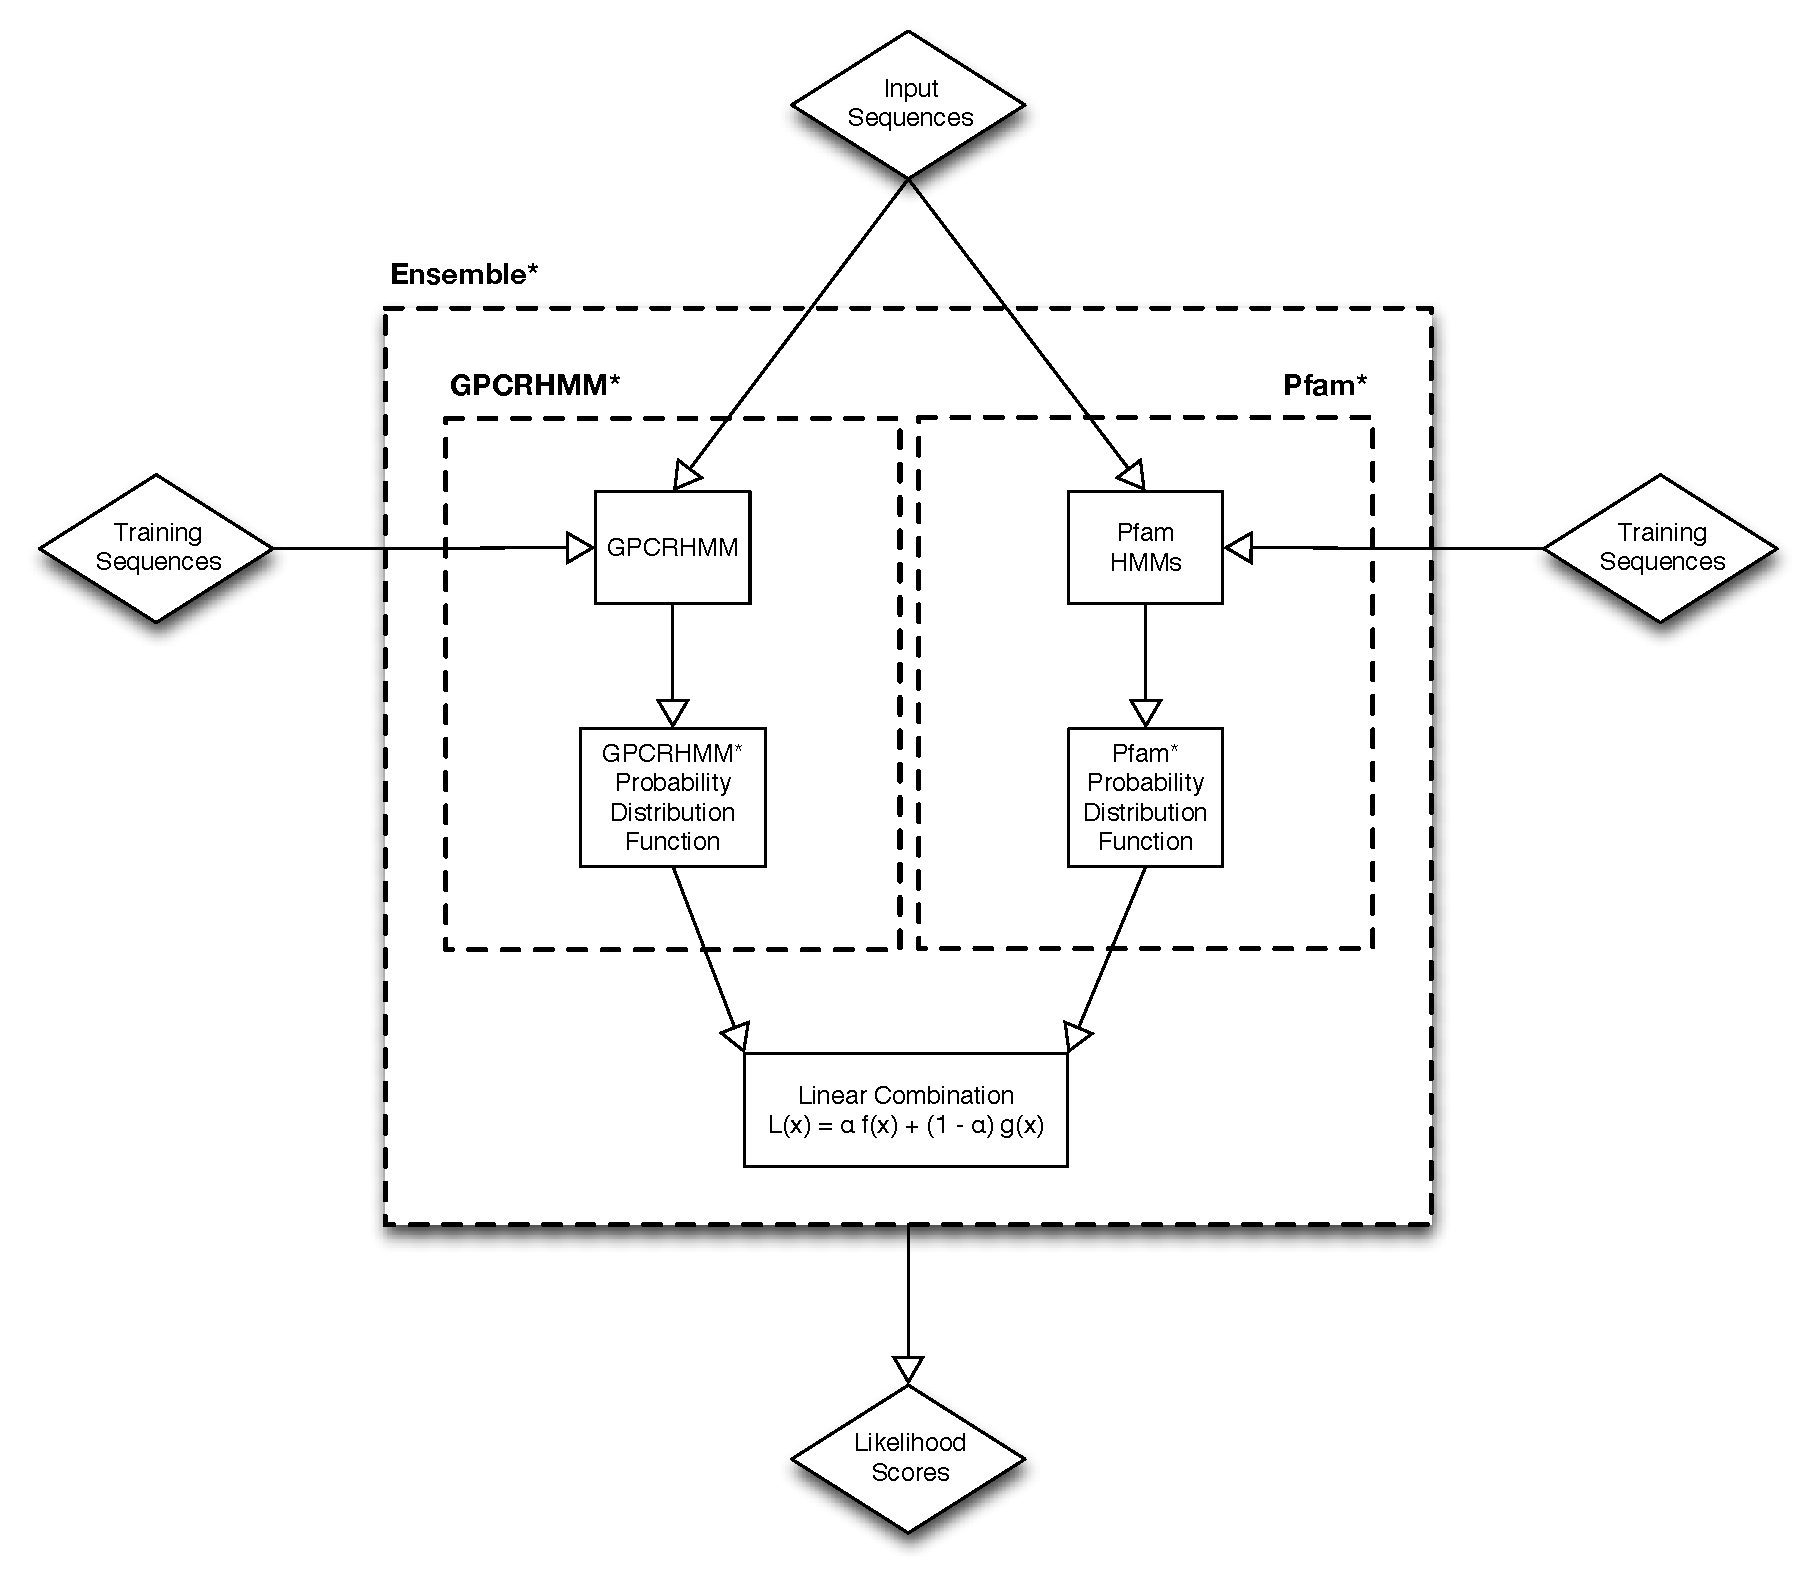
\includegraphics[width=0.8\textwidth]{figures/gpcr_classifier/ensemble-diagram.eps}
  
Flowchart describing the Ensemble*, GPCRHMM*, and Pfam* classifiers.  The diamonds represent sequences, while the rectangles represent steps of the classifiers.  The dashed rectangles describe to which classifiers the components belong. The input sequences are the sequences to be classified, while the training sequences are sequences which have known designations of either GPCR or not GPCR.
\label{fig:ensemble-diagram}
\end{figure}

\begin{figure}[H]
  \centering
  \caption{ROC Curve for Combined Data Set}
  \includegraphics[width=0.8\textwidth]{figures/gpcr_classifier/combined_ensembl_roc.eps}
  
ROC Curve Comparing Classifier Performance on Combined Data Set. The dashed (GPCRHMM*), dotted (Pfam*), and solid (Ensemble*) curves represent the relationship between the percentage of training set GPCRs correctly predicted (true positives) plotted against the percentage of sequences miss-classified as GPCRs (false positives) by the classifiers as the likelihood score threshold was decreased from 1 (accepting nothing) to 0 (accepting everything). GPCRHMM (diamond), Pfam (circle), and PredCouple (square) only produce true/false predictions for each sequence and hence are represented as single points.
\label{fig:combined-roc-curve}
\end{figure}

\begin{figure}[H]
  \centering
  \caption{ROC Curves for Individual Organisms}
\includegraphics[width=0.8\textwidth]{figures/gpcr_classifier/organism_ensembl_roc.eps}

ROC Curves Comparing Classifier Performance on Individual Organisms.  For each ROC curve, the classifiers were trained on five of the organisms and then evaluated on the sixth organism (given in the title).  The solid (Ensemble*), dashed (GPCRHMM*), and dotted (Pfam*) lines represent the relationship between the percentage of correctly predicted training set GPCRs (true positives) and the percentage of incorrectly predicted non-GPCRS (false positives) as the likelihood score threshold is decreased from 1 (accept nothing) to 0 (accept everything).  GPCRHMM (diamond), Pfam (circle), and PredCouple (square) only produce true/false predictions for each sequence and hence are represented as single points.
\label{fig:individual-roc-curves}
\end{figure}

\begin{figure}[H]
  \centering
  \caption{GPCR Validation Pipeline}
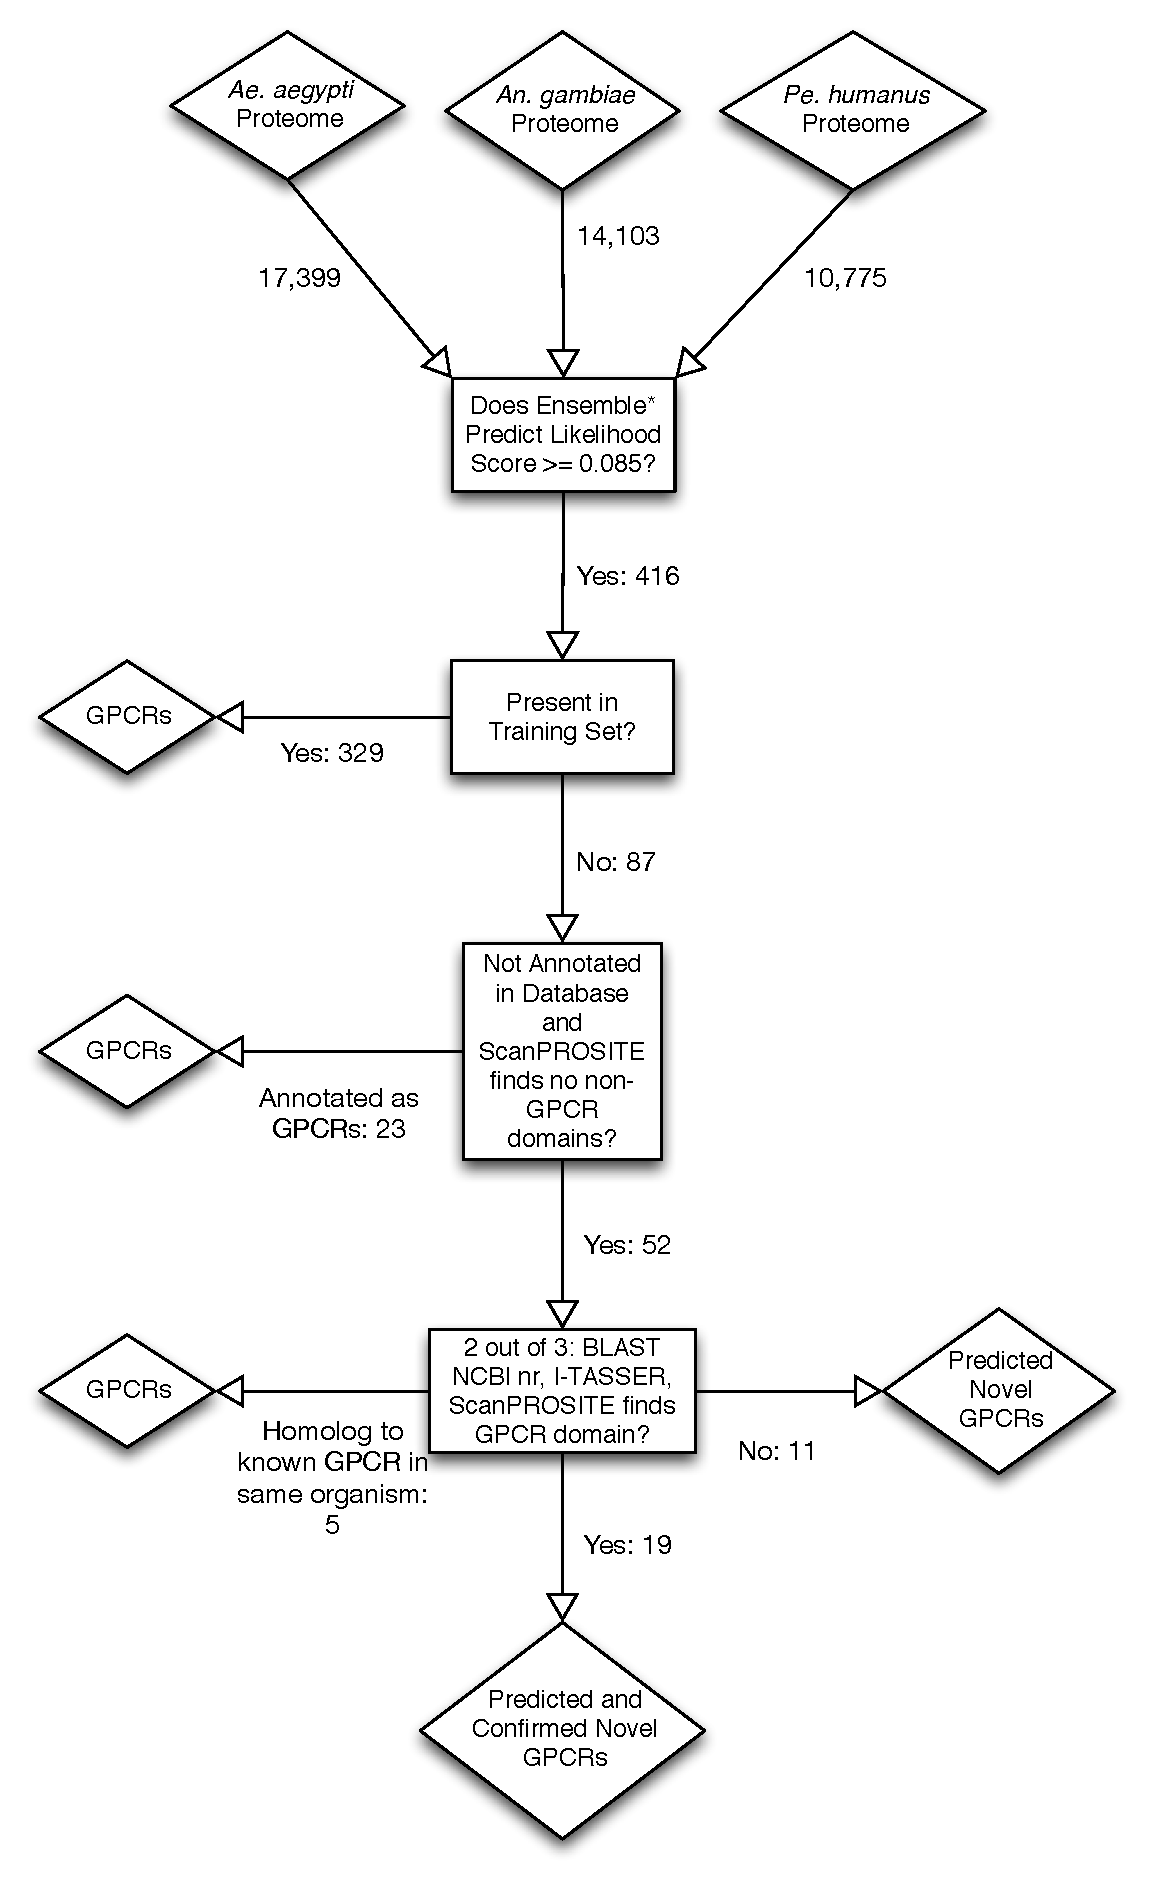
\includegraphics[width=0.6\textwidth]{figures/gpcr_classifier/validation-pipeline.eps}

GPCR Validation Pipeline.  Diamonds indicate input and output sequences.  Rectangles represent the validation programs and filters.  Arrows indicate the movement of sequences and are labeled with the number of sequences that passed from one validation step to the next.  Numbers for sequences that were identified as something other than GPCRs are not shown.  The first filter identifies sequences which are annotated as GPCRs in the database and removes any sequences which were annotated as something other than GPCRs or were identified by ScanPROSITE as having non-GPCR domains.  The second filter uses a combination of the BLAST hits, I-TASSER results, and identification of GPCR domains by ScanPROSITE to categorize the final 52 predicted but unconfirmed sequences.
\label{fig:validation-pipeline}
\end{figure}

\begin{figure}[H]
  \centering
  \caption{Distribution of Newly-Discovered GPCR Sequences}
  \includegraphics[width=0.8\textwidth]{figures/gpcr_classifier/summary-independent-validation.eps}
  
Distribution of the newly-discovered vector GPCR sequences according to their GPCR status for each vector species.
\label{fig:summary-independent-validation}
\end{figure}

\section{Tables}


\begin{table}[H]
%  \centering
  \caption{\uppercase{Data Set Sources and Construction}}
  \small
  \begin{tabular}{| l | p{5cm} | p{5cm} |}
    \hline
    \textbf{Organism} & \textbf{Predicted Proteome Source and Version} & \textbf{Training Set Source} \\ \hline
    \emph{Ae. aegypti} & VectorBase, v. AaegL1.2 & VB and GPCRDB annotations \\ \hline
    \emph{An. gambiae} & VectorBase, v. AgamP3.5 & \cite{Hill2002}, VB and GPCRDB annotations \\ \hline
    \emph{Ap. mellifera} & Beebase, v. Pre-Release 2\_OGS & GPCRDB annotations \\ \hline
    \emph{Dr. melanogaster} & Flybase, v. 5.29 & Flybase and GPCRDB annotations \\ \hline
    \emph{Ho. sapiens} & Ensembl, v. 37.59 & \cite{Zhang2006}, Ensembl and GPCRDB annotations \\ \hline
    \emph{Pe. humanus} & VectorBase, v. 1.2 & VB and GPCRDB annotations \\ \hline
  \end{tabular}
  \label{tab:data-sources}
  
\end{table}

\begin{table}[H]
%  \begin{center}
  \caption{\uppercase{Classifiers' True Positive Rates for Different False Positive Rates}}
  \small
  \begin{tabular}{| l | p{2.25cm} | p{2.25cm} | p{2.25cm} | p{2.25cm} | p{2.25cm} |}
    \hline
    \textbf{Classifier} & \multicolumn{5}{c |}{\textbf{True Positive Rate (TPR)}} \\ \hline
               & GPCRHMM's FPR (0.0061) & PredCouple's FPR (0.0066) & Pfam's FPR (0.0067) & FPR where Ensemble*'s TPR Plateaus (0.01) & Best for all FPRs $\leq$ 0.01 \\ \hline
    Ensemble*  & 87\%                   & 89\%                      & 89\%                & 91\%                                      & 91\% \\ \hline
    GPCRHMM    & 81\%                   & --                        & --                  & --                                        & 81\% \\ \hline
    GPCRHMM*   & 81\%                   & 81\%                      & 81\%                & 83\%                                      & 83\% \\ \hline
    Pfam       & --                     & --                        & 82\%                & --                                        & 82\% \\ \hline
    Pfam*      & 80\%                   & 80\%                      & 80\%                & 80\%                                      & 80\% \\ \hline
    PredCouple & --                     & 86\%                      & --                  & --                                        & 86\% \\ \hline
  \end{tabular}
  %  \end{center}
  
  Percentage of training set GPCRs correctly predicted (true positive rates) for fixed percentages of sequences misclassified as GPCRs (false positive rates) are given.  The false positive rates (FPR) of GPCRHMM, PredCouple, Pfam, and at which Ensemble*'s true positive rate plateaus were chosen to provide the most direct comparisons between the classifiers.
  \label{tab:ensemble-results}
\end{table}

\begin{table}[H]
%\begin{center}
\caption{\uppercase{Number of Test Set Sequences Found / Missed by Species}}
\small
\begin{tabular}{| c | c | c | c | c |}
\hline
\textbf{Species (Total Sequences)}                 & \multicolumn{4}{ c |}{\textbf{Number of Sequences Found / Missed}*} \\ \hline
                                 & GPCRHMM    & Pfam        & PredCouple  & Ensemble*   \\ \hline
\emph{Ae. aegypti} (134)      & 73 / 61    & 111 / 23    & 101 / 33    & \textbf{122 / 12} \\ \hline
\emph{An. gambiae} (137)      & 105 / 32   & 115 / 22    & 113 / 24    & \textbf{122 / 15} \\ \hline
\emph{Ap. mellifera} (56)     & 45 / 11    & 54 / 2      & 54 / 2      & \textbf{56 / 0}  \\ \hline
\emph{Dr. melanogaster} (195) & 176 / 19   & 156 / 39    & 180 / 15    & \textbf{185 / 10} \\ \hline
\emph{Ho. sapiens} (892)      & 759 / 133  & 712 / 180   & 778 / 114   & \textbf{807 / 85} \\ \hline
\emph{Pe. humanus} (103)      & 72 / 31    & 89 / 14     & 86 / 17     & \textbf{95 / 8}  \\ \hline
Vectors (374)                    & 250 / 124  & 315 / 59    & 300 / 74    & \textbf{339 / 35} \\ \hline
Total (1517)                     & 1230 / 287 & 1237 / 280  & 1312 / 205  & \textbf{1387 / 130} \\ \hline
\end{tabular}
%\end{center}

The number of test set sequences each classifier identified (found) and was unable to identify (missed) as GPCRs are given by species, vectors, and total. GPCRHMM, Pfam, and Predcouple were run using default settings. For Ensemble*, sequences with a positive likelihood score were considered to predicted GPCRs.  The best results are in bold.
\label{tab:missed-sequences}
\end{table}

\newpage

\begin{longtable}{| l | l | p{2cm} | p{3.25cm} | p{3.5cm} |}
\caption{\label{tab:novel-gpcrs} \uppercase{Newly-Discovered GPCRs Identified by Ensemble*}} \\ \hline
\textbf{Sequence ID} & \textbf{Species} & \textbf{Prediction Likelihood Value} & \textbf{Evidence} & \textbf{BLAST Sequence Name}
\endfirsthead
\hline
\textbf{Sequence ID} & \textbf{Species} & \textbf{Prediction Likelihood Value} & \textbf{Evidence} & \textbf{BLAST Sequence Name} \endhead
\caption*{Sequences were predicted using the Ensemble* classifier.  Independent validation was performed using ScanPROSITE, I-TASSER, and homology to GPCRs in other organisms as determined by a BLAST search of the NCBI nr database.  Status as a newly-discovered GPCR was contingent upon identification by the Ensemble* classifier and the existence of no contrary evidence, while confirmed GPCRs also had to be validated by at least two independent methods.}\\
\endlastfoot
\hline
    AAEL013430-PA & \emph{Ae. aegypti} & 0.346 & ScanPROSITE and BLAST and I-TASSER & putative GPCR class a orphan receptor 5 \\ \hline
    AAEL000818-PA & \emph{Ae. aegypti} & 0.188 & ScanPROSITE and BLAST & class C metabotropic glutamate-like G-protein coupled receptor GPRmgl4, putative \\ \hline
    AGAP002229-PA & \emph{An. gambiae} & 0.691 & ScanPROSITE and BLAST & serotonin receptor \\ \hline
    AGAP004930-PA & \emph{An. gambiae} & 0.658 & ScanPROSITE and BLAST and I-TASSER & G protein coupled receptor \\ \hline
    AGAP000383-PA & \emph{An. gambiae} & 0.480 & ScanPROSITE and BLAST & G protein coupled receptor \\ \hline
    AGAP005229-PA & \emph{An. gambiae} & 0.440 & ScanPROSITE and BLAST and I-TASSER & G protein coupled receptor \\ \hline
    AGAP000606-PA & \emph{An. gambiae} & 0.411 & ScanPROSITE and BLAST & alpha-2 adrenergic receptor \\ \hline
    AGAP013324-PA & \emph{An. gambiae} & 0.409 & ScanPROSITE and BLAST & G protein-coupled receptor \\ \hline
    AGAP008703-PA & \emph{An. gambiae} & 0.278 & ScanPROSITE and BLAST and I-TASSER & G protein coupled receptor \\ \hline
    AGAP008237-PA & \emph{An. gambiae} & 0.250 & BLAST and I-TASSER & G-protein coupled receptor 143 \\ \hline
    AGAP011320-PA & \emph{An. gambiae} & 0.236 & ScanPROSITE and BLAST and I-TASSER & Beta-3 adrenergic receptor \\ \hline
    AGAP012824-PA & \emph{An. gambiae} & 0.167 & ScanPROSITE and BLAST and I-TASSER & tachykinin receptor \\ \hline
    AGAP011646-PA & \emph{An. gambiae} & 0.112 & ScanPROSITE and BLAST & class C metabotropic glutamate-like G-protein coupled receptor \\ \hline
    PHUM074100-PA & \emph{Pe. humanus} & 0.375 & ScanPROSITE and BLAST & Frizzled-7 \\ \hline
    PHUM010590-PA & \emph{Pe. humanus} & 0.342 & ScanPROSITE and I-TASSER & PREDICTED: cadherin EGF LAG seven-pass G-type receptor 3-like \\ \hline
    PHUM423330-PA & \emph{Pe. humanus} & 0.289 & ScanPROSITE and I-TASSER & N/A \\ \hline
    PHUM447490-PA & \emph{Pe. humanus} & 0.250 & ScanPROSITE and I-TASSER & neuropeptide receptor A31 \\ \hline
    PHUM618870-PA & \emph{Pe. humanus} & 0.208 & ScanPROSITE and I-TASSER & G protein-coupled receptor \\ \hline
    PHUM128700-PA & \emph{Pe. humanus} & 0.167 & ScanPROSITE and I-TASSER & G-protein coupled receptor \\ \hline
    AAEL005994-PA & \emph{Ae. aegypti} & 0.278 & Unconfirmed & uridine cytidine kinase i \\ \hline
    AAEL002694-PA & \emph{Ae. aegypti} & 0.250 & Unconfirmed & transmembrane protein 87A \\ \hline
    AAEL000851-PA & \emph{Ae. aegypti} & 0.217 & Unconfirmed & N/A \\ \hline
    AAEL010852-PA & \emph{Ae. aegypti} & 0.214 & Unconfirmed & Transmembrane protein 145 \\ \hline
    AGAP000130-PA & \emph{An. gambiae} & 0.430 & Unconfirmed & PREDICTED: latrophilin 2-like \\ \hline
    AGAP005356-PA & \emph{An. gambiae} & 0.423 & Unconfirmed & PREDICTED: alpha-1A adrenergic receptor-like \\ \hline
    AGAP011701-PA & \emph{An. gambiae} & 0.400 & Unconfirmed & GPRmgl4 \\ \hline
    AGAP004783-PA & \emph{An. gambiae} & 0.227 & Unconfirmed & neuropeptide receptor A16 \\ \hline
    AGAP007896-PA & \emph{An. gambiae} & 0.141 & Unconfirmed & sprinter \\ \hline
    PHUM596180-PA & \emph{Pe. humanus} & 0.476 & Unconfirmed & transmembrane protein 145 \\ \hline
    PHUM288590-PA & \emph{Pe. humanus} & 0.136 & Unconfirmed & N/A \\ \hline

\end{longtable}




\chapter{Ranking Biologically-Interesting SNPs in Incipient Species of Malaria Vectors using Random Forests}

\section{Abstract}
  Half of the world's population are at risk for malaria infection through vectors such as the mosquitoes \emph{Anopheles gambiae} and \emph{Anopheles coluzzii}.  Having recently diverged, the two species differ in feeding and mating habits as well as insecticide resistence but cannot be differentiated visually. Identifying genetic differences between the two species is key to understanding the biological differences and designing effective population-control efforts.
  Random Forests have been used in bioinformatics literature to identify subsets of genetic markers which describe phenotypic differences in studies as diverse as cancer and diabetes. 
  We use numerical experiments to illustrate the susceptibility of Random Forests to multiple sources of bias if not used with care, which affect variable importance score accuracy.
  We describe solutions to correct for bias and demonstrate that Random Forests can identify biologically-meaningful biallelic SNPs in insect vectors.

\section{Introduction}
The accumulation of genetic differences within separate populations may result in new species. Genetic differences between long-separated species often have macroscopic genomic differences such as re-ordered genes that are relatively easy to detect. During the early stages of speciation, however, genetic differences are often subtle, occurring in the form of differences in allele frequencies or combinations thereof. For example, the apple maggot \emph{Rhagoletis pomonella} separated from \emph{Rhagoletis zepheria} no more than two centuries ago, but allele frequencies likely changed rapidly \cite{Egan2015}.  Another classic example of recent speciation are the malaria vectors \emph{An. gambiae} and \emph{An. coluzzii} that were difficult to distingish genetically even after whole genome sequencing \cite{Lawniczak2010}. Tools and methods for identifying identifying genetic differences are valuable to efforts aiming to molecularly characterize such closely related species and ultimately understand underlying causes of speciation in these model systems.

Genetic differentiation of insects, however, faces several challenges. Although the genome sizes can be relatively small compared to human, collecting and sequencing enough samples is costly for these communities.  Further, many of these species have very little linkage disequilibrium (LD), for which single nucletide polymorphisms (SNPs) tend to be the primary feature (as opposed to larger haplotype blocks in species like human). Combined, currently available data sets tend to be ``wide'' with many features and few samples \cite{Lawniczak2010, Egan2015, Fontaine2015}.

Given the lack of LD, the typical method as applied to insect population genomics involve calculating multiple univariate statistics such as $F_{ST}$, nucleotide diversity ($\pi$), and Tajima's $D$ \cite{Fontaine2015}. Relatively diverged regions are isolated by atypical values, usually visualized across the genome \cite{Egan2015, Fontaine2015}. Due to the relatively small amount of information per SNP, a common strategy is to look at genome intervals (windows) in an attempt to amplify signal. Window-based analysis is able to find interactions between nearby SNPs but not larger interacting regions, especially in the absence of a previously competed reference genome \cite{Egan2015}.

Random Forests (RFs) offer an attractive alternative to more traditional techniques \cite{Breiman1999}. RFs are a versatile machine learning method that can be used for classification (supervised learning), variable selection, regression, and clustering (unsupervised learning).  RFs are able to utilize heterogenous features types such as real numbers or integers, categories, and ordinals. RFs also tend to perform well on data sets with numerous unlinked features such as genome-based SNPs with little LD \cite{Meng2009}.

RFs have started to see adoption across a range of problems in computational biology.  D\'{\i}az-Uriarte, et al. applied RFs to gene selection and classification from microarray data, finding that RFs perform in the case of a large number of noisy features \cite{Diaz-Uriarte2006}. Jiang, et al. successfully applied RFs to the classification of microRNA precursors \cite{Jiang2007}. Chen, et al. used RFs to predict protein-protein interactions \cite{Chen2005}. Kandaaswamy, et al. used RFs to identify anti-freeze proteins from sequence-derived features. RF clustering has been used by Shi, et al. to classify tumors from microarray data \cite{Shi2005}. Lin, et al. and Wu, et al. used RFs to identify DNA-binding proteins \cite{Lin2011}. Jiang, et al. applied RFs to predict SNP interactions associated with Age-related Macular Degeneration in a genome-wide associated study \cite{Jiang2009}. Lunetta, et al. also applied RFs to predicting SNP interactions in a large-scale association study \cite{Lunetta2004}.  Liu, et al. applied RFs to identifying protein-RNA binding sites \cite{Liu2010}. Moore, et al. reviewed computational challenges in genome-wide association studies, arguing for Random Forests as one solution \cite{Moore2010}.

Researchers have begun to identify challenges associated with using RFs for bioinformatics problems and extensions to RF methods. Strobl, et al. identified issues with bias in RF variable importance scores associated with categorical variables and bootstrap resampling of samples during training and proposed a new method called ``cforest'' \cite{Strobl2007}. Nicodemus, et al. analyzed bias present in RF permutation-based variable importance measures \cite{Nicodemus2010}. To overcome identified issues, Strobl, et al. proposed the Conditional Random Forest method \cite{Strobl2008}. Altmann, et al. proposed using permutation importance as variable importance measure that avoids bias present in the more traditional Gini importance measure \cite{Altmann2010}. Calle, et al. compared two common variable importance measures, mean decrease accuracy and mean decrease Gini, finding that mean decrease Gini is more stable in the face of small perturbations \cite{Calle2011}. Amaratunga, et al. proposed using weights so that features are not sampled uniformally in splits, calling the method Enriched Random Forests \cite{Amaratunga2008}.

We consider the problem of apply RFs to challenging whole-genome studies of early speciation of insects. We use simulated data sets to demonstrate that RFs are susceptible to multiple sources of bias, in line with previous work by Strobl, et al \cite{Strobl2007, Strobl2008, Nicodemus2010} and Altmann, et al. \cite{Altmann2010}. Unlike the previous work, we describe a solutions that can be used with common ``out-of-the-box'' implementations of decision trees. We apply our solutions to ranking SNPs, which we validate by identifying SNPs associated with incipient speciation of insect vectors.  Our workflow is implemented in and available through an open-source software package written in Python using the Numpy and scikit-learn libraries.


\section{Methods and Implementation}


\subsection{Variable Transformation}
The first stage is conversion of input SNP data into a data representation suitable for Random Forest construction.  Aranyani expects a VCF file containing $M$ phased SNP variants for $N$ individuals and a file mapping the individuals' IDs to populations.  Aranyani converts the input VCF file into a feature matrix consisting of Boolean-valued columns, known as ``one-hot encoding.'' For each SNP, a Boolean-valued (represented as 0s and 1s) column is created for each nucleotide value (A, T, C, G) present in the individuals.  Unknown nucleotides (X) are represented by 0 (false) values in all of the columns.  The four columns for each haploid are mutually-exclusive -- only one column can have a 1 (true) value.  One-hot encoding is used to prevent bias in the machine learning models due to varying sizes of the categorical variables.

Table~\ref{tab:snp-examples} contains examples of SNP values for three individuals with the resulting feature matrix in Table~\ref{tab:features-example}.  The SNPs are labeled by triplets of chromosome, position, and haploid.  The first SNP (1, 1, 1) is represented by two columns ((1, 1, 1, A) and (1, 1, 1, T)) in the feature matrix since the individuals have two nucleotides (A and T) between them. Individuals 1 and 3 have 1s in column 1 (1, 1, 1, A) and 0s in column 2 (1, 1, 1, T) of the features matrix since their SNP values are A, while individual 2 has a 0 in column 2 (1, 1, 1, A) and a 1 in column 2 (1, 1, 1, T).

Note that unknown nucleotides (X) do not receive their own columns.  In cases where individuals have an unknown nucleotide, 0s are placed in all columns for that SNP.  For example, individual 3 has 0s in columns 4 (1, 10, 1, C), 5 (1, 10, 1, G), and 6 (1, 10, 2, A) since the nucleotides are unknown for those SNPs.

\begin{table}[h!]
  \begin{center}
    \begin{tabular}{ c c c c c }
      \hline
      \textbf{Individual} & \textbf{(1, 1, 1)} & \textbf{(1, 1, 2)} & \textbf{(1, 10, 1)} & \textbf{(1, 10, 2)} \\ \hline
      1 & A & T & C & X \\
      2 & T & T & G & A \\
      3 & A & T & X & X \\
    \end{tabular}
  \end{center}
  \caption{Examples of SNP values for three individuals.  The SNPs are labeled by triplets of (chromosome, position, haploid).}
  \label{tab:snp-examples}
\end{table}

\begin{table}[h!]
  \begin{center}
    \begin{tabular}{ c c c c c c c}
      \hline
      \textbf{Individual} & \textbf{(1, 1, 1, A)} & \textbf{(1, 1, 1, T)} &\textbf{(1, 1, 2, T)} & \textbf{(1, 10, 1, C)} & \textbf{(1, 10, 1, G)} &\textbf{(1, 10, 2, A)} \\ \hline
      1 & 1 & 0 & 1 & 1 & 0 & 0 \\
      2 & 0 & 1 & 1 & 0 & 1 & 1 \\
      3 & 1 & 0 & 1 & 0 & 0 & 0 \\
    \end{tabular}
  \end{center}
  \caption{Feature matrix for three individuals in Table~\ref{tab:snp-examples}.  The features are labeled by quartets of (chromosome, position, haploid, nucleotide value).}
  \label{tab:features-example}
\end{table}

After populating the feature matrix, the columns that have same value either because there are no SNPs or all individuals have the same genotype are removed.  Filtering prevents errors in the machine learning models, reduces memory and disk usage, and improves run times.  We use two criteria for filtering columns. SNPs where individuals all have the same value result in a single feature column with all 1s.  Such a SNP offers no information for distinguishing between individuals and are filterd out.  For an example, see SNP column 2 (1, 1, 2) in Table~\ref{tab:snp-examples} represented by feature column 3 (1, 1, 2, T) in Table~\ref{tab:features-example}.

Likewise, SNPs with only one known nucleotide value are also filtered out. The feature columns may contain both 1s and 0s (in the case of unknown nucleotides).  For example, see SNP column 4 (1, 10, 2) in Table~\ref{tab:snp-examples} represented by feature column 6 (1, 10, 2, A) in Table~\ref{tab:features-example}.  Although the values would distinguish between individuals, we would be classifying individuals based on unknown information -- we do not want the machine learning models to associate an unknown value (X) as different from a known value (T).  This could lead to errors in classifications since the unknown value might actually be one of the known values.

Table~\ref{tab:filtered-features-example} gives the result of filtering the feature matrix in Table~\ref{tab:features-example}. Columns 3 (1, 1, 2, T) and 6 (1, 10, 2, A) were removed since they match the first and second criteria, respectively.

\begin{table}[h!]
  \begin{center}
    \begin{tabular}{ c c c c c }
      \hline
      \textbf{Individual} & \textbf{(1, 1, 1, A)} & \textbf{(1, 1, 1, T)} & \textbf{(1, 10, 1, C)} & \textbf{(1, 10, 1, G)} \\ \hline
      1 & 1 & 0 & 1 & 0 \\
      2 & 0 & 1 & 0 & 1 \\
      3 & 1 & 0 & 0 & 0 \\
    \end{tabular}
  \end{center}
  \caption{Filtered feature matrix for three individuals in Table~\ref{tab:snp-examples}.  The features are labeled by quartets of (chromosome, position, haploid, nucleotide value).}
  \label{tab:filtered-features-example}
\end{table}

\subsection{Ranking SNPs}
SNPs are ranked by their ``variable (feature) importance'' scores computed from the decision trees in a Random Forest model.  A decision tree encodes how combinations of feature values uniquely identify one class (group) of individuals from another.  Decision trees are generated by choosing a feature and thresholding its values into two groups at every split in the tree.  The particular feature and threshold are chosen to maximize the sorting individuals by class according to an objective function such as the Gini impurity. Trees are grown until either a maximum depth is reached, a number of samples in a leaf node have reached a given minimum, or leaf nodes have homogenous values (all individuals are from the same class).

A Random Forest is an ensemble of decision trees with uses bagging of individuals and random subsampling of features.  For every decision tree in a Random Forest, the individuals are resampled (known as bootstrapping or bagging) from the original set of individuals and a randomly-chosen subset of features are chosen for training the tree. The addition of the two sampling procedures increases variation among the trees and enables exploring a wide range of feature combinations.

After training the random forest, we compute the SNP importance scores from the features' variable importance scores, calculated for each feature by averaging and scaling their objective function values.  Features used in nodes closer to the top of tree generally have higher variable importance scores.  Features' variable importance scores are averaged across all of the trees in the Random Forest.  The variable importance scores for each SNP are calculated by averaging the variable importance scores of the corresponding features.  For example, the variable importance score for the SNP of column 1 (1, 1, 1) in Table~\ref{tab:snp-examples} would be calculated as the average of the scores for features of columns 1 (1, 1, 1, A) and 2 (1, 1, 1, T) in Table~\ref{tab:filtered-features-example}.  SNPs with importance score of zero (i.e., SNPs that haven't been sampled by the Random Forests) are filtered out.  The remaining SNPs are ranked according to their importance scores.  SNPs with higher importance scores are higher in the rankings.

\textcolor{red}{Provide example of calculations}


\subsection{Effect of Tree Counts on SNP Importance Score Convergence}
Parameters for the Random Forests include the number of trees, the number of features to sample, the maximum depth, and the minimum number of individuals needed to split a node.  We use a minimum split size of two and set the maximum depth to a large number.  Since the number of individuals used in biological work is very small (tens of individuals), the trees tend to be quite small, utilizing only tens of features and with depths of $<$10.  We found that randomly sampling $\sqrt{n_{features}}$ leads to the fastest convergence (in terms of number of trees) of the SNP importance scores.  This leaves the number of trees as the only parameter that the user must set.  More trees leads to less variance in the SNP importance scores.

We provide an analysis approach to guide the user in determining the number of trees needed for the SNP importance scores to converge.  We sweep over the number of trees, training two Random Forest models for each parameter value.  SNPs' importance scores are computed from each model and ranked.  The top ranked SNPs from each model, for a set of thresholds provided by the user, are compared to identify the percentage of SNPs in common.  If the two models are converged, 100\% of the SNPs should be the same for any ranking threshold. The common percentage of SNPs for various thresholds as a function of the number of trees are reported in a plot (see Figure~\ref{fig:ranking-convergence-analysis}).  The user can use the plot as a guide for choosing the number of trees.

\subsection{Software Implementation}
Aranyani is implemented in Python using the Numpy, Scikit Learn, and Matplotlib libraries.  Aranyani has an extensive set of unit tests to prevent defects and make changes easier to make.  The Random Forests functionality is provided by Scikit Learn. Numpy memory-mapped arrays are used to support feature matrices larger than available RAM.   Aranyani is available under the Apache License v2 at \url{http://www.github.com/rnowling/aranyani}.

\textcolor{red}{extend when software is developed}

\section{Results}

\subsection{Bias from Encoding of Categorical Variables}
Analysis by Strobl, et al. \cite{Strobl2007} and Altmann, et al. \cite{Altmann2010} found that variable importance scores from Random Forests were biased towards categorical variables with more categories.  Genomic data primarily consists of categorical variables, making categorical variable bias an important issue.  We re-created Altmann, et. al.'s simulation studies to study the effect of encoding schemes on variable importance of categorical variables.  We randomly generated 100 datasets with 1000 samples and uninformative 31 categorical variables with 2-32 categories each.  The values of the categorical variables were sampled from an uniform distribution so that each category had an equal chance of being chosen and no correlation with the output labels. Random Forests with 100 trees were trained on each dataset and used to compute variable importance scores.

We evaluated two encoding schemes: integer encoding and one-hot encoding.  Under the integer encoding scheme, each of the 31 categorical variables was encoded as a column in the feature matrix with the categories represented as integers starting from 0.  In one-hot encoding, each category variable of $N$ categories is encoded as $N$ columns of 0's and 1's.  The columns are mutually exclusive such that only one of the columns can be ``hot,'' or have value of 1 for each sample.  The resulting feature matrix had 527 columns.  When computing the variable importance score for each one-hot encoded categorical variable, we averaged the variable importance scores from the columns associated with that variable.

In our simulation studies, we found that the bias observed by Altmann, et al. \cite{Altmann2010} may have been due to the encoding scheme used; we observed the bias reported by Altmann, et al. with integer encoding but not one-hot encoding. We would expect the variable importance scores to be equal across all of the variables since each variable is equally uninformative.  As the box plots in Figure~\ref{fig:integer} demonstrate, variables with more categories have higher variable importances with integer encoding.   When using one-hot encoding, however, the variable importances are uniform (see Figure~\ref{fig:one-hot}), regardless of the number of categories.  Our results suggest that the bias observed by Altmann, et al. may have been a result of the encoding scheme and can be corrected by using one-hot encoding.

% integer encoding used commonly in bioinformatics.  nucleic acids, amino acids, etc.

\subsection{Bias from Unknown Genotypes}
Due to sequencing and assembly challenges of the genomes of non-model organisms, SNPs for some samples may have unknown genotypes.  We generated synthetic data to analyze the effect of missing data on the variable importance scores.  We simulated 12 biallelic SNPs with possible values of A/A, A/T, and T/T.  Each SNP was encoded as two features, giving the number of As and Ts respectively.  For example, A/A becomes (2, 0), A/T becomes (1, 1), and T/T becomes (0, 2).  The SNPs are organized into four groups of three.  The first three SNPs are chosen from a uniform distribution and uncorrelated with the output labels.  The remaining three groups of SNPs have 100\%, 75\%, and 50\% probabilities, respectively, of being correlated with the output label. To simulate the effect of missing data, we zeroed out the features of the first, second, and third SNP in each group for 0, 10, and 20 randomly-chosen individuals.  We generated 100 datasets with 100 samples each and trained a RF with 100 trees on each dataset.  

The variable importance scores are plotted in Figure~\ref{fig:missing-data}.  The variable importance scores for features with no missing data are shown in Figure~\ref{fig:missing-data-none}, while the variable importance scores with the missing data are shown in Figure~\ref{fig:missing-data-missing}.  Each sequential pair of variables correspond to a SNP.  For example, variables 1 and 2 correspond to SNP 1. Variables 7-12 correspond to the SNPs with perfect correlation to the output label, 13-18 correspond to SNPs with 75\% correlation, and SNPs 19-24 correspond to the variables with 50\% correlation.

Figure~\ref{fig:missing-data-missing} demonstrates that removing data for 10 (or 10\%) and 20 (or 20\%) of the individuals leads to significant decreases in the variable importance scores.  Variables 7-8 have significantly higher variable importance scores than variables 9-10 and 11-12. In our control (Figure~\ref{fig:missing-data-none}), all of these variables have the same importance scores.

Unknown genotypes are a characteristic of the data set, not the underlying biology.  Penalizing SNPs with important biological function due to missing data for some individuals may not desirable. Imputation is a commonly-used approach in machine learning to overcome the problem of missing data.  The most popular approach is to filling in missing data with an average of the known values from individuals in the same class.  Since we're using discrete data, we chose to evaluate using the mode, or most common value, for imputation.  Simulations were carried in the same manner as for the missing data, but individuals' missing values were replaced with the most common value from individuals in the same class.  The resulting variable importance scores are shown in Figure~\ref{fig:missing-data-imputed}.  Imputing the data with the mode ``recovers'' the original variable importance scores, demonstrating that imputation can be used successfully to overcome bias due to missing data.

\subsection{Effect of Number of Variables and Correlated Variables on Variable Importance Scores} \label{sec:correlated}
The variable importance scores are calculated at two levels.  For each tree, the mean decrease in impurity is calculated for each feature used.  Features that are not used in a tree receive a mean decrease of 0 for that tree.  The variable importance scores are then calculated by taking the average of the mean decreases in impurity for each feature across all of the trees.

\[
VIM_f = \frac {1} {N_t} \sum_{t=1}^{N_t} \bar{\Delta}_{f, t}
\]

where $\bar{\Delta_{f, t}}$ is the mean decrease in impurity of feature $f$ for tree $t$ and $N_t$ is the total number of trees.

In the case where we have a large number of features but a small number of samples, only a small number of features will be used in each tree.  As a result, the feature importance scores will be down-weighted by a large number of 0's and vary with the number of trees used.

We used synthetic data set to evaluate the effect of the number of variables on feature importance scores.  We randomly generated data sets of 10 samples with 5, 10, and 25 uncorrelated binary variables.  The output labels were sampled uniformally from $\{0, 1\}$.  Variable importance scores were computed from Random Forests with 100 trees.  We ran 100 simulations.  The distributions of variable importance scores are plotted in Figure~\ref{fig:var-count}.  As the number of variables increased from 5 to 10 and 25, the variable importance score for each variable decrease.

Correlation between informative variables introduces another source of bias. We used simulations to evaluate the effect of variable correlation on variable importance scores. We randomly generated data sets of 10 samples with 25 binary variables.  The data sets had 1, 10, and 25 features with values correlated with the output label and each other. The output labels were sampled uniformally from $\{0, 1\}$. Variable importance scores were computed from one Random Forest with 100 trees per simulation.  We ran 100 simulations.

The distributions of variable importance scores and number of times each feature was used in a tree are plotted in Figure~\ref{fig:corr-1}.  As the number of correlated features increased, the variable importance scores of each feature decreased.  The number of times each feature was selected also decreased.  Since each tree only needed to selected a subset of the correlated features, the number of selected variables decreased, down-weighting the variable importance scores.

Our analysis suggest that the bias in variable importance scores for correlated variables are due to each variable being chosen less frequently as the number of variables increase.  For our use case, the number of informative features is large and the number of features used per tree is small.  As such, informative features are not chosen more often than they are chosen, causing their variable importance scores to be down-weighted by a large number of zeros (the default variable importance scores when a variable is not selected).

\textcolor{red}{are scores of correlated variables distinguishable from uncorrelated variables even with large numbers of variables?}

\subsection{Bias from Re-sampling} \label{sec:resampling}
Random Forests employ ``bootstrap aggregation,'' or bagging, to improve classification accuracy on classifiers which are unstable \cite{Breiman1996}.  Unstable classifiers like decision trees may generate models that differ greatly when small changes are made to the training set.  Bagging compensates by re-sampling the original training set for each tree trained, thus accounting for variations in possible data sets frequencies.  Bagging employs two steps: 1) bootstrap resampling of the original training set to create a new training set for each decision tree and 2) employing a majority-vote scheme for classification in which each decision tree gets one vote.

With small sample sizes such as 10 or 20 samples, individual samples are frequently excluded from re-sampled data sets.  Consider a variable with values that are split along class lines for all but one or two samples. Due to the high frequency with which the one or two samples with confounding values will be excluded from the re-sampled data sets, the variable will have a mean decrease impurity of 1 from some of the decision trees. 

For our use case, our goal is to obtain variable importance scores that are accurate relative to the genotypes present in the original population; classification accuracy is not our concern.  If we observe a genotype in one of the samples, we know that genotype is present in the original population. We don't want to exclude any of the observed genotypes, even if those genotypes have a very low frequency of occurrence in the original population.  As a consequence, bagging can cause the variable importance scores of variables with one or two samples with confounding values will be larger than expected, and thus, biased.

We propose ``constrained bagging'' in sampled copies are added to the original training set rather than replacing samples.  Each re-sampled training set contains the original training set plus zero or more additional samples.   With zero re-samples, there is no variance in the re-sampled training sets.  With a small number of the re-samples, the sample occurrences have a high probability of being skewed relative the frequencies of the original training set.  As the number of re-samples increases, the distribution of sample occurrences have a high probability of being equal to the frequencies fo the original training set.  As a result, the number of re-samples controls the variance in the sample occurrence counts, a property of multinomial models.

We evaluated the effects of bagging and contrained bagging on mean decreases in impurity using simulations.  We randomly generated data sets of ten samples with none binary variables. The data sets had two classes with five samples assigned to each.  Seven of the variables were uncorrelated -- values were chosen uniformally from $\{0, 1\}$. One of the variables was correlated with the output label.  And lastly, one of the variables was correlated with the output label for all but one sample, which had a value equal to the output label for the other class.  Distributions of mean decrease in impurities were calculated using 10,000 decision trees.

Figure~\ref{fig:bagging-bias} shows the distribution of mean decreases in impurity for a confounded variable with bagging and contrained bagging with 0, 10, 100, and 1000 additional re-samples.  With bagging, the mean decrease in impurity is calculated as 1 for 10\% of the decision trees, evidence of the situation we want to avoid.  With zero additional re-samples, the mean decrease in impurity is frequently in the range $[0.65, 0.70)$ but does not incorporate the possible variance in the frequencies of the genotypes in the underlying population.  By adding 10, 100, and 1000 re-samples, the sample frequencies are allowed to fluctuate to estimate possible frequency distributions that could be present in the underlying population.  With a smaller number of re-samples, the impurities vary significantly, while the impurity distribution begins to converge to that with no re-samples when using a large number of re-samples.

\subsection{Determining Number of Trees Needed for Stable Rankings}

\subsection{Software}
We combined one-hot encoding, genotype imputation, constrained bagging, and our methodology for determining the number of trees needed for stable ranking of SNPs to form a workflow for ranking SNPs.  We implemented our workflow in a Python software packaged called ``Asaph'' using the Numpy and scikit-learn libraries.  Asaph is available under the open-source Apache License v2 at \url{https://github.com/rnowling/asaph}.

To reduce run times and memory usage, we employed dictionary compression on the columns of the feature matrix. Duplicate variables are grouped and replaced with a single instance.  A mapping between the original variables and replacement variable is maintained.  We can set the variable importance score for each variable in a duplicated set equal to the score of the single remaining variable.

When applied to the SNPs of \emph{An. funestus}, dictionary compression reduced the number of features from 4,472,916 to 49,924, a reduction of 98.9\%.   This suggests that biological data sets may have a significant number of duplicated variables.  By reducing the number of variables to 1\% of the original size, run times were $\approx100 \times$ faster, reduced from hours to minutes.

\subsection{Application to \emph{An. gambiae} and \emph{An. coluzzii}}
We applied ``Asaph'' to analysis of SNPs from the malaria vectors \emph{An. gambiae} and \emph{An. coluzzii}, two incipient species of mosquitoes.

\begin{table}[h!]
  \begin{center}
    \begin{tabular}{ c c c p{8cm} }
      \hline
      \textbf{Chromosome} & \textbf{Position} & \textbf{Score} & \textbf{Notes} \\ \hline
      2L & 25396564 & 0.00032 &  \emph{resistance to dieldrin (Rdl)} gene associated with insecticide resistance (\textcolor{red}{Lawnziak et al, 2009})\\
      2L & 11568165 & 0.00032 &  \\
      2L & 21707904 & 0.00031 &  \\
      X  & 18853272 & 0.00122 &  \\
      X  & 19789366 & 0.00121 &  \\
      X  & 20141128 & 0.00121 & Intron 2-3 of Armadillo segment polarity protein (AGAP001043-RA) (\textcolor{red}{Neafsey et al, 2009})\\
      X  & 18927357 & 0.00119 & Intron 1-2 of cuticular protein (AGAP000986-RA) \\
      X  & 15271290 & 0.00118 &  \\
      X  & 14564483 & 0.00118 &  \\
      X  & 18441856 & 0.00117 & Intron 2-3 of nicotinic acetylcholine receptor subunit alpha 7 (AGAP000962-RA) (\textcolor{red}{Neafsey et al, 2009})\\
      X  & 19820035 & 0.00115 &  \\
      X  & 19513702 & 0.00112 & Intron 5-6 of notch gene homolog 1 (AGAP001015-RA) (\textcolor{red}{Neafsey et al, 2009})\\
    \end{tabular}
  \end{center}
  \caption{Fixed Differences from the top-ranked SNPs for 2L and X chromosomes of \emph{An. gambiae} vs \emph{An. coluzzii}.}
  \label{tab:filtered-features-example}
\end{table}

\subsection{Application to \emph{An. funestus}}
\emph{An. funestus} mosquitoes, along with \emph{An. gambiae}, are a major vector of malaria in Africa \textcolor{red}{cite}. Recent studies have shown that \emph{An. funestus} has two chromosomal forms, Folonzo and Kiribina.  We analyzed 1,874,475 SNPs from 10 samples, five of each chromosomal form, using our Asaph software.  We used dictionary compression and 1 million trees.

Variable importance scores of all of the SNPs, sorted by rankare shown in Figure~\ref{fig:funestus-all}.  We distinguish between the 7,156 SNPs (red) that trivially separate the two forms (the genotypes of each form are disjoint) and the rest, which we call ``confounding.''  We note that the Random Forests are unable to distinguish between trivial SNPs; any small differences in variable importance scores are a result of small differences in the number of times each SNP was sampled.  Trivial SNPs include fixed differences as well as SNPs in which one form may have two genotypes.  Methods like $F_{ST}$ downweight SNPs with variation within a population, allowing them to distinguish between fixed differences and other forms that trivial SNPs can take.

We observe several gaps in variable importances of groups of SNPs.  The trivial SNPs have variable importance scores $> 10^{-3}$.  A smaller block of 503 confounding SNPs has VIMs between $4\times 10^{-4}$ and $6\times 10^{-4}$.  A third, larger block of 26,078 SNPs have VIMs in the range of $3\times 10^{-4}$ and $1\times 10^{-4}$.  




Resistance to pyrethroid insecticides has been observed in \emph{An. funestus}, affecting population control efforts \textcolor{red}{cite}.   

\section{Discussion}

\section{Conclusion}

\section{Figures}

\pagebreak

\begin{figure}[H]
  \centering
  \begin{subfigure}[b]{0.45\textwidth}
    \includegraphics[width=\textwidth]{figures/random_forests/rf_bias_integer}
    \caption{Integer Encoded}
    \label{fig:integer}
  \end{subfigure}
  ~
  \begin{subfigure}[b]{0.45\textwidth}
    \includegraphics[width=\textwidth]{figures/random_forests/rf_bias_onehot}
    \caption{One-Hot Encoded}
    \label{fig:one-hot}
  \end{subfigure}
  \caption{Comparison of effect of encoding schemes for categorical variables on variable importance scores. The variables have randomly-chosen values with no correlation with output labels and 2-32 categories.}
  \label{fig:encoding-schemes}
\end{figure}

\begin{figure}[H]
  \centering
  \begin{subfigure}[b]{0.45\textwidth}
    \includegraphics[width=\textwidth]{figures/random_forests/rf_missing_data_none}
    \caption{No Missing Data}
    \label{fig:missing-data-none}
  \end{subfigure}
  ~
  \begin{subfigure}[b]{0.45\textwidth}
    \includegraphics[width=\textwidth]{figures/random_forests/rf_missing_data}
    \caption{Missing Data}
    \label{fig:missing-data-missing}
  \end{subfigure}
  ~
  \begin{subfigure}[b]{0.45\textwidth}
    \includegraphics[width=\textwidth]{figures/random_forests/rf_missing_data_imputed_mode}
    \caption{Missing Data Imputed with Mode}
    \label{fig:missing-data-imputed}
  \end{subfigure}
  \caption{Effect of missing data on variable importance scores.}
  \label{fig:missing-data}
\end{figure}

\begin{figure}[H]
  \centering
  \begin{subfigure}[b]{0.45\textwidth}
    \includegraphics[width=\textwidth]{figures/random_forests/rf_variable_count_bias_5.png}
    \caption{5 Uninformative Variables}
    \label{fig:var-count-5}
  \end{subfigure}
  ~
  \begin{subfigure}[b]{0.45\textwidth}
    \includegraphics[width=\textwidth]{figures/random_forests/rf_variable_count_bias_10.png}
    \caption{10 Uninformative Variables}
    \label{fig:var-count-10}
  \end{subfigure}
  ~
  \begin{subfigure}[b]{0.45\textwidth}
    \includegraphics[width=\textwidth]{figures/random_forests/rf_variable_count_bias_25.png}
    \caption{25 Uninformative Variables}
    \label{fig:var-count-25}
  \end{subfigure}
  \caption{Distributions of variable importance scores with 5, 10, and 25 uninformative variables.}
  \label{fig:var-count}
\end{figure}

\begin{figure}[H]
  \centering
  \begin{subfigure}[b]{0.45\textwidth}
    \includegraphics[width=\textwidth]{figures/random_forests/rf_correlated_1_0_1.png}
    \caption{1 Correlated Variable}
    \label{fig:corr-1-1}
  \end{subfigure}
  ~
  \begin{subfigure}[b]{0.45\textwidth}
    \includegraphics[width=\textwidth]{figures/random_forests/rf_correlated_1_0_1_feature_counts.png}
    \caption{1 Correlated Variable}
    \label{fig:corr-1-1-counts}
  \end{subfigure}
  ~
  \begin{subfigure}[b]{0.45\textwidth}
    \includegraphics[width=\textwidth]{figures/random_forests/rf_correlated_1_0_10.png}
    \caption{10 Correlated Variables}
    \label{fig:corr-1-10}
  \end{subfigure}
  ~
  \begin{subfigure}[b]{0.45\textwidth}
    \includegraphics[width=\textwidth]{figures/random_forests/rf_correlated_1_0_10_feature_counts.png}
    \caption{10 Correlated Variables}
    \label{fig:corr-1-10-counts}
  \end{subfigure}
  ~
  \begin{subfigure}[b]{0.45\textwidth}
    \includegraphics[width=\textwidth]{figures/random_forests/rf_correlated_1_0_25.png}
    \caption{25 Correlated Variables}
    \label{fig:corr-1-25}
  \end{subfigure}
  ~
  \begin{subfigure}[b]{0.45\textwidth}
    \includegraphics[width=\textwidth]{figures/random_forests/rf_correlated_1_0_25_feature_counts.png}
    \caption{25 Correlated Variables}
    \label{fig:corr-1-25-counts}
  \end{subfigure}
  ~
  \caption{Analysis of variables from generated data sets with 1, 10, and 25 out of 25 variables perfectly correlated with the output label. The left-hand side figures are distributions of variable importance scores. Right-hand side figures are number of trees using each variable.}
  \label{fig:corr-1}
\end{figure}

\begin{figure}[H]
  \centering
  \begin{subfigure}[b]{0.45\textwidth}
    \includegraphics[width=\textwidth]{figures/random_forests/bagging_bias_bagging_hist.png}
    \caption{Bagging}
    \label{fig:bagging-bias-bagging}
  \end{subfigure}
  ~
  \begin{subfigure}[b]{0.45\textwidth}
    \includegraphics[width=\textwidth]{figures/random_forests/bagging_bias_no_bagging_hist.png}
    \caption{Constrained Bagging, 0 Resamples}
    \label{fig:bagging-bias-constrained-0}
  \end{subfigure}
  ~
  \begin{subfigure}[b]{0.45\textwidth}
    \includegraphics[width=\textwidth]{figures/random_forests/bagging_bias_constrained_bagging_hist_10.png}
    \caption{Constrained Bagging, 10 Resamples}
    \label{fig:bagging-bias-constrained-10}
  \end{subfigure}
  ~
  \begin{subfigure}[b]{0.45\textwidth}
    \includegraphics[width=\textwidth]{figures/random_forests/bagging_bias_constrained_bagging_hist_100.png}
    \caption{Constrained Bagging, 100 Resamples}
    \label{fig:bagging-bias-constrained-100}
  \end{subfigure}
  ~
  \begin{subfigure}[b]{0.45\textwidth}
    \includegraphics[width=\textwidth]{figures/random_forests/bagging_bias_constrained_bagging_hist_1000.png}
    \caption{Constrained Bagging, 1000 Resamples}
    \label{fig:bagging-bias-constrained-1000}
  \end{subfigure}
  ~
  \caption{Distributions of mean decreases in impurity when using bagging and constrained bagging with 0, 10, 100, and 1000 additional re-sampled instances.}
  \label{fig:bagging-bias}
\end{figure}

\begin{figure}[H]
  \centering
  \begin{subfigure}[b]{0.45\textwidth}
    \includegraphics[width=\textwidth]{figures/random_forests/snp_counts}
    \caption{Sampled SNP Counts}
    \label{fig:ranking-counts}
  \end{subfigure}
  ~
  \begin{subfigure}[b]{0.45\textwidth}
    \includegraphics[width=\textwidth]{figures/random_forests/common_snps}
    \caption{Common SNPs by Rank}
    \label{fig:ranking-common}
  \end{subfigure}
  \caption{Analysis of sampled SNPs and common SNPs by rank.}
  \label{fig:ranking}
\end{figure}

\begin{figure}[H]
  \centering
  \begin{subfigure}[b]{0.45\textwidth}
    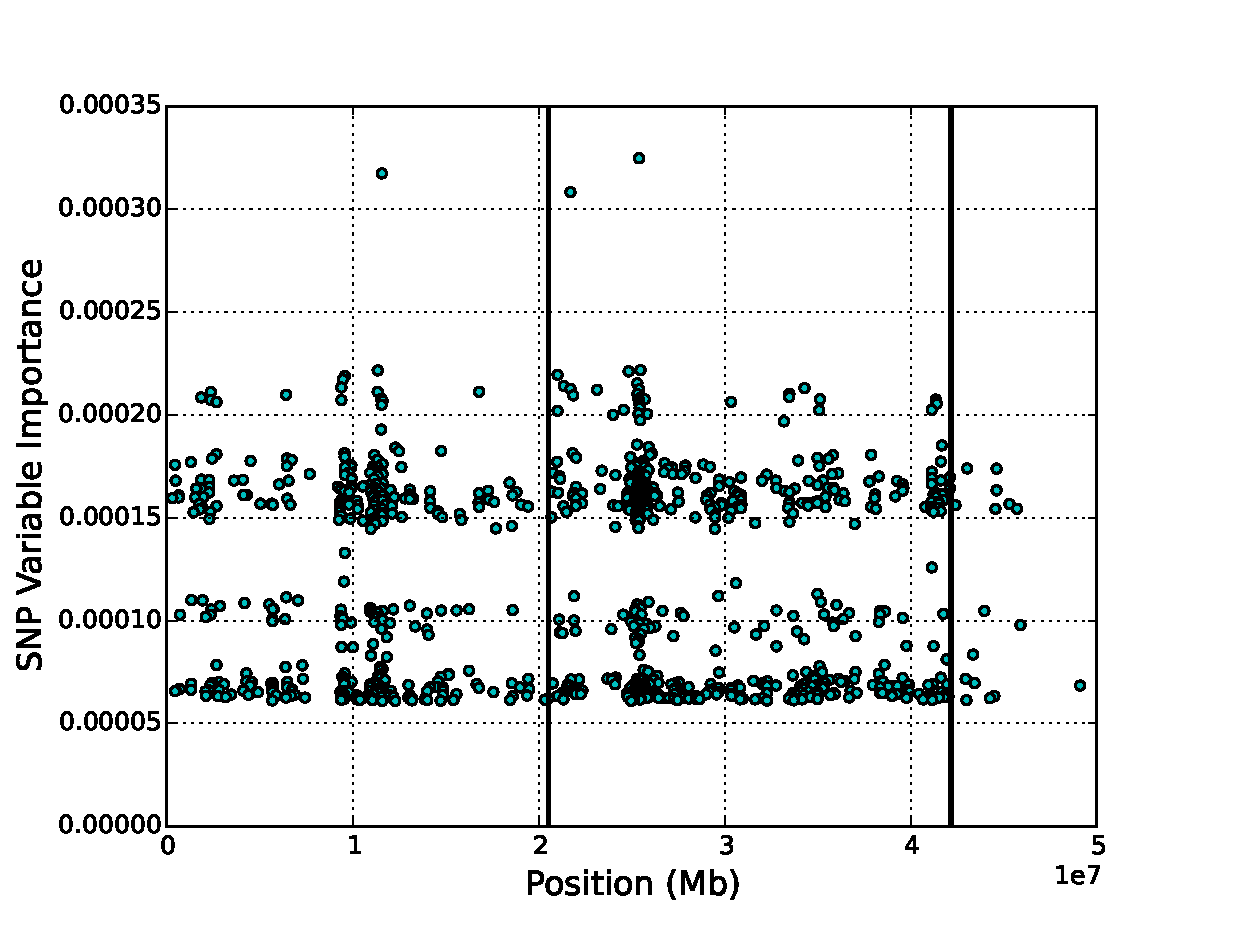
\includegraphics[width=\textwidth]{figures/random_forests/anopheles_2L_importances}
    \caption{Chromosome 2L}
    \label{fig:anopheles-2l}
  \end{subfigure}
  ~
  \begin{subfigure}[b]{0.45\textwidth}
    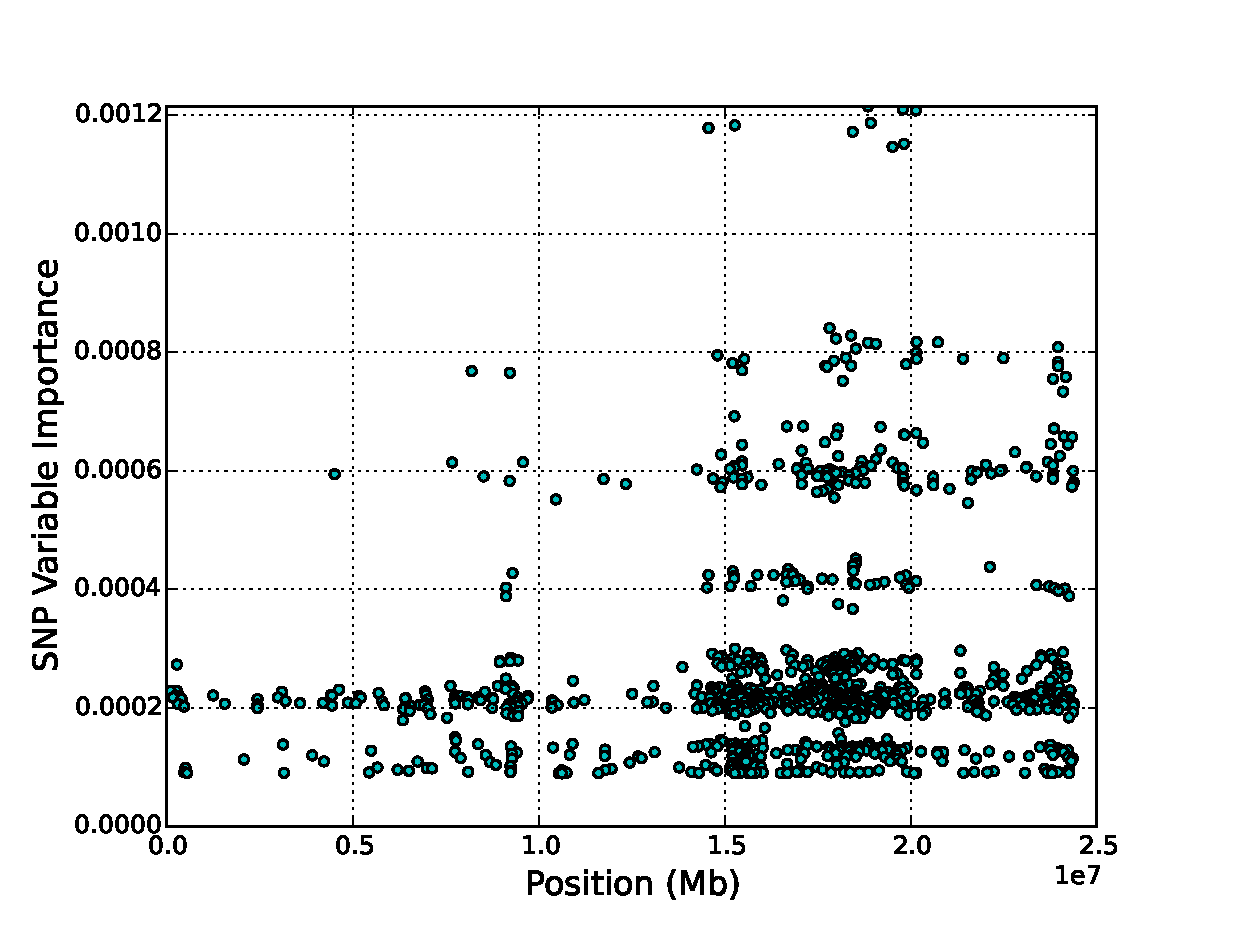
\includegraphics[width=\textwidth]{figures/random_forests/anopheles_X_importances}
    \caption{Chromosome X}
    \label{fig:anopheles-x}
  \end{subfigure}
  \caption{SNP Variable Importances for 2L and X chromosomes of \emph{An. gambiae} vs \emph{An. colluzzi}.  The cyan circles indicate the SNP variable importances.  The black lines bound the 2La inversion.}
  \label{fig:ranking-convergence-analysis}
\end{figure}

\begin{figure}[H]
  \centering
  \begin{subfigure}[b]{0.45\textwidth}
    \includegraphics[width=\textwidth]{figures/random_forests/funestus_ranks_10resamples_1000000trees_scores}
    \caption{All SNPs}
    \label{fig:funestus-all}
  \end{subfigure}
  ~
  \begin{subfigure}[b]{0.45\textwidth}
    \includegraphics[width=\textwidth]{figures/random_forests/funestus_ranks_10resamples_1000000trees_scores_subset}
    \caption{VIMs $> 10^{-4}$}
    \label{fig:funestus-thresholded}
  \end{subfigure}
  \caption{Variable importance scores of \emph{An. funestus} SNPs.}
  \label{fig:funestus}
\end{figure}

\chapter{\uppercase{Conclusion}}
The thesis of this dissertation is that machine learning techniques can be used to augment or replace traditional, domain-specific methods in bioinformatics.  To argue this thesis, we presented several contributions:

\begin{enumerate}
\item Chapter 2: A comparative genomic analysis of two sand fly species, \emph{Lu. longipalpis} and \emph{P. papatasi}, and differential expression analysis of genes from \emph{Lu. longipalpis} females under sugar-fed, blood-fed, and infected blood-fed conditions. Our analysis of the sand flies illustrates several challenges arising in the study of insect vectors, including incomplete genome assemblies and high rates of genome shuffling.
\item Chapter 3: We evaluated several popular methods (GPCRHMM, PredCouple, and Pfam GPCR Hidden Markov Models (HMMs)) for identifying G Protein-Coupled Receptors (GPCRs) in insect vector genomes. We demonstrated improved prediction performance on insect vector GPCRs from combining multiple classifiers into an ensemble, an application of a technique popularized by machine learning.
\item Chapter 4: We demonstrated that Random Forests, a popular machine learning technique, can be applied to ranking biallelic SNPs in the context of insect vector population genetics while also describing multiple sources of bias and their solutions.  We implemented our workflow in a new software package called Asaph using Python and scikit-learn.
\end{enumerate}

We believe we believe our contributions are significant, we also believe that there are several interesting avenues for future work related to and enabled by the work described in this dissertation.

As the number of sequenced genomes increases, not only in insect vector biology but in other areas such as personalized medicine, analysis software capable of scaling to larger data sets will be needed.  Researchers will need to consider not only issues of model accuracy but engineering processes for reducing development time and transitioning proof-of-concept implementations into production systems usable by industry. Such efforts should be supported by empirical evaluations of the practical utility, from a software engineering perspective, of machine learning libraries and distributed (``big data'') platforms such as Apache Spark in bioinformatics application development.

Secondly, we successfully demonstrated that machine learning techniques could replace domain-specific techniques in at least one problem domain: population genetics. Further work could evaluate the applicability of machine learning to other problem domains within bioinformatics.

Lastly, further studies are needed to address proper application apply machine learning methods in bioinformatics to avoid bias. There are a number of open questions about how to handle small sample sizes (to avoid overfitting), data representation, and how best to handle missing data.  As these questions are addressed, best practices and appropriate workflows can be established and codified through the availability of software and documentation.

Ultimately, we hope to inspire other researchers to think about the accuracy of their models along with employing pragmatic software engineering strategies; both are important to enabling bioinformatics to achieve significant gains in improving human health.



\appendix
\chapter{\uppercase{A Domain-Driven, Generative Data Model for BigPetStore}}
\epigraph{\textit{At the end of my fourth year, I took a full-time position as software engineer at Red Hat, Inc. and dropped from being a full-time Ph.D. student to a part-time student.  Shortly after starting, I designed a generative model to simulate customer transactions for a fictional chain of pet stores, with the intention of enabling testing and realistic demos of open-source ``big data'' platforms.  In collaboration with Jay Vyas, my friend, Red Hat colleague, and collaborator from my time at the University of Connecticut Health Center (UCHC), I described and published the model in the conference paper copied below.  I decided to include the paper here, even though it is not part of my dissertation, because it serves as additional evidence of my capacity to conduct and publish independent research.  More sentimentally, the work serves as a tribute to my academic research career, connecting, through Jay, the beginning of my academic research career at UCHC to its end as I defend my Ph.D. at Notre Dame and begin a new career at Red Hat.}}

\section{Abstract}
Generating large amounts of semantically-rich data for testing big data workflows is paramount for scalable performance benchmarking and quality assurance in modern machine-learning and analytics workloads.  The most obvious use case for such a generative algorithm is in conjunction with a big data application blueprint, which can be used by developers (to test their emerging big data solutions) as well as end users (as a starting point for validating infrastructure installations, building novel applications, and learning analytics methods).

We present a new domain-driven, generative data model for BigPetStore, a big data application blueprint for the Hadoop ecosystem included in the Apache BigTop distribution. We describe the model and demonstrate its ability to generate semantically-rich data at variable scale ranging from a single machine to a large cluster.  We validate the model by using the generated data to answer questions about customer locations and purchasing habits for a fictional targeted advertising campaign, a common business use case.

\section{Introduction}
Big data applications process large, dynamic, multidimensional data sets with the general goal of information and knowledge extraction.  With the wide variety of big data tools available and lagging documentation, both developers and users of big data systems benefit from the availability of realistic example applications.  For developers, such applications are useful for testing, benchmarking, and evaluating design choices; for users, example applications provide starting points for learning methods, developing their own applications, and implementing new analytics workflows.

BigPetStore is one such big data application blueprint built around processing transaction data for a fictional chain of pet stores.  BigPetStore targets the Hadoop \cite{Hadoop} ecosystem with examples implemented for loading, cleaning, aggregating, and performing analytics on data using Hive \cite{Thusoo2010}, Pig \cite{Olston2008,Gates2009}, and Mahout \cite{Mahout}. BigPetStore has been incorporated into the open-source Apache BigTop distribution \cite{BigTop}, where it is used for testing and as a reference application. One of BigPetStore's key features is the ability to scale from a single machine to a large cluster, making it easy to develop projects on a local machine and transfer the application to a large cluster for production testing.

To achieve the project's goals of providing high-quality, realistic examples, BigPetStore requires semantically-rich, complex data. At its core, BigPetStore relies on a generative data model for producing synthetic transaction data. Despite the growing number of real data sets now publically available, synthetic data generators have a number of advantages for BigPetStore over real data sets. The synthetic data generator can be packaged with BigPetStore, avoiding the cost, time, and infrastructure needed to host, transfer, and store large data sets. Synthetic data generators are scalable, allowing the user to choose how much data to generate -- a requirement for supporting BigPetStore's goal of running on both single machines and large clusters.  Licensing and privacy issues are avoided with the use of synthetic data sets. And lastly, the generated data can be customized by the user, allowing the user to generate data with specific criteria amenable to testing.  For example, a user may generate transactions from a small number of purchasable items so that clustering results can be easily visualized.

A variety of approaches for generating synthetic data sets exist.  TeraGen and the Intel Hadoop Benchmark Suite \cite{Huang2010} are popular tools that can generate data sets quickly and at any scale, but the resulting data is semantically-void and not useful for much more than simple benchmarks.  Multiple frameworks exist for generating synthetic data sets that satisfy relational database schemas \cite{Ghazal2013,Rabl2011a,Frank2012,Rabl2011,Gray1994,Bruno2005,Hoag2007}, and several approaches even provide domain-specific languages \cite{LogSynth,Bruno2005,Hoag2007} for specifying additional constraints (such as which distributions to sample from and allow for modeling basic relationships between fields using simple arithmetic equations \cite{Alexandrov2012}).

Recent work has addressed some aspects of the need for more dynamic data set generation: Arasu, et al. \cite{Arasu2011} demonstrated that constraint-solving techniques could be used as an alternative to procedural approaches. Such frameworks allow for reproducing the structural properties of real data, but the frameworks are not expressive enough to describe the dynamic generation processes and latent variables that would be needed to embed the desired informational complexity and rich semantics needed for BigPetStore's analytics examples.

Realizing the difficulty in creating a generic framework capable of modeling the semantics of real data, recent work \cite{Alexandrov2013} has focused on generating synthetic data sets that satisfy characteristics learned from real reference data. Such approaches appear promising but will need to overcome the difficulties of accurately training models, especially on raw data instead of features.

Until such purely generic methods reach maturity, BigPetStore's needs are best met by a customized, domain-driven model. Another example of such a model is The Information Discovery and Analysis System (IDAS) Data Set Generator (IDSG) \cite{Jeske2005,Lin2006}. IDSG was developed to test the effectiveness of IDASs in identifying potential terrorism threat scenarios using synthetic data.  Like BigPetStore, the developers of IDSG needed to avoid licensing restrictions and privacy issues associated with real data.

BigPetStore's current model has been used successfully to generate terabytes of synthetic data and is used regularly for testing in Apache BigTop, showcasing the value of the approach.  The current model is limited, however, in its ability to generate data that is semantically rich, limiting progress on BigPetStore's goals of providing realistic analytics examples.

In this work, we present a new domain-driven model and simulation method for BigPetStore.  Compared with BigPetStore's previous data generator, our model and implementation can generate data which contains geospatial, temporal, and quantitative features, similar to the type of data which businesses and organizations might typically encounter.  Combining the features of the TeraGen (scalability)  and MovieLens \cite{MovieLens} (semantically rich) input data sets commonly used for big data benchmarking, we present a synthetic data set generator which can be used to benchmark lower level tasks (such as sorting) as well as higher level tasks (such as clustering, recommending, and search indexing) at arbitrary scale.  To demonstrate that the model generates data with desirable properties, we performed an example analysis designed to guide a fictional advertising campaign (a typical business use case). The model's implementation was made available as open source software.

\section{Overview of Model \& Simulation Procedures}
Our generative model combines various well-known mathematical modeling techniques to simulate the factors affecting customers' purchasing habits.  Each part of the model is derived from \emph{ab initio} assumptions.  In several cases, real data is used to parameterize parts of the model. 

\subsection{Description of Generated Data}
The model generates data for four types of records: stores, customers, transactions, and transaction items (Figure~\ref{fig:relational-data-model}).  Store records contain both a unique identifier and a location in the form of a 5-digit zip code. Customer records consist of a unique identifier, a name, and a location given as a 5-digit zip code. Transaction records consist of a transaction identifier, a customer identifier, a store identifier, and a time given in days since the beginning of the simulation. Transaction item records contain a transaction identifier and an item description.  The item description is a list of key-value pairs stored as a string.  Key-value pairs are used since item characteristics differ depending on the type of item.  For example, dog food has a brand, a flavor, a size (in lbs), and a per-unit cost, while poop bags have a brand, a color, a count, and a per-unit cost.

\begin{figure}[!t]
  \centering
  \caption{\uppercase{Relational Data Model for Generated Data}}
  \includegraphics[width=3.5in]{figures/bigpetstore/transactions_data_model.eps}
  \label{fig:relational-data-model}
\end{figure}

\subsection{Generation of Stores}
The locations of the stores are modeled by a probability density function (PDF) that gives the probability that a store's location is the given zip code. We designed the PDF to give to zip codes in high-population, high-income areas the highest probabilities. The PDF is composed of two individual PDFs. One PDF determines the probability of each zip code as the population of that zip code over the total population:

\begin{equation*}
p(\text{location}=z | \text{population}(z)) = \frac{\text{population}(z)}{\sum_{i} \text{population}(i)}
\end{equation*}

The second PDF scales the probabilities of the zip codes by their incomes.  The zip code with the highest-income has a probability $s$-times larger than that of the lowest-income zip code. The values in-between are interpolated using an exponential function:

\begin{equation*}
p(\text{location}=z | \text{income}(z)) = s ^ {\big( \frac{\text{income} - \min_i{\textrm{income}(i)}} {\max_i{\textrm{income}(i)} - \min_i{\textrm{income}(i)}} - 1 \big)}
\end{equation*}

The combined PDF is given as: 

\begin{align*}
p(\text{location}=z) = &Z p(\text{location}=z | \text{population}(z)) \\
&p(\text{location}=z | \text{income}(z))
\end{align*}

where $Z$ is the normalization factor.  Given the small size ($\approx$30,000 zip codes) of the data set, $Z$ can be found directly by iterating over all of the zip codes and summing the scores. The population and household income data for the zip codes were taken from from the U.S. Census American Community Survey \cite{ACS}.  The stores' locations are generated by sampling zip codes from the PDF.

\subsection{Generation of Customers}
For each proposed customer location zip code $z$, we compute the distance $d_m(z)$ between $z$ and each store's zip code $s_z$ to find the closest store.  The zip codes' latitudes and longitudes (taken from the Zip Code Database Project \cite{Zips}) are used to compute the distances. Each zip code $z$ is assigned a weight $w_z$ according to its distance $d_m(z)$ to the nearest store using an exponential distribution with the average distance $\beta$:

\begin{align*}
&w_z = \beta^{-1} \exp(-\beta^{-1} \, d_m(z)) \\
&d_m(z) = \min_{s_z} \, d(z, s_z)
\end{align*}

The customer's zip code is chosen by sampling from the zip codes with the probabiltiy of choosing each zip code $z$ proportional to its weight $w_z$.

Names are generated using data from the Name Database\cite{NameDB}. Each record in the database gives a name, a weight, and flag indicatings if the name can be used as a first name, a last name, or both.  PDFs generated for the first and last names using the weights.  The customer's name is generated by sampling a first name and a last name from each PDF respectively.

We determine the number of pets $N_p$ each customer has by sampling from a discrete uniform distribution of integers. We then sample the number of dogs $N_d$ as a discrete uniform distribution of integers between 0 and $N_p$.  The remaining number of pets are assigned to be cats.

\begin{align*}
N_c = N_p - N_d \\
N_d \sim U(0, N_p) \\
N_p \sim U(1, b)
\end{align*}

\subsection{Simulation of Transactions}
A transaction simulation is run for each customer. The transaction's store is set to the store located closest to the customer.  Transaction times are generated from a Monte Carlo process that proposes transaction times based on the usage of the customer's items and Poisson processes modeling the amount of time between the customer visiting the store and running out of the items (Section~\ref{sec:transaction-times}).  The purchased items are generated by a Hidden Markov Model (HMM) parameterized by the transaction time and amount of time remaining for the items in the customer's inventory (Section~\ref{sec:transaction-purchases}).

\begin{figure}[!t]
  \centering
  \caption{\uppercase{Flowchart of Transaction Monte Carlo Simulation}}
  \includegraphics[width=3.5in]{figures/bigpetstore/transaction_simulation.eps}
  \label{fig:trans_sim}
\end{figure}

\subsection{Simulation of Transaction Times} \label{sec:transaction-times}
Transaction times are simulated using a Monte Carlo method (Figure~\ref{fig:trans_sim}).  The usage over time of each item category is simulated. Items categories are groups of items which are interchangeable such as ``dry dog food,'' ``dry cat food,'' and ``kitty litter.'' The time between the customer's visit to the store to buy more items in each category and the exhaustion time of that item category is modeled using a Poisson process. Proposed transaction times for each item category are computed based on the exhaustion time and time sampled from the Poisson process. The earliest transaction time is taken as the overall proposed transaction time.  The probability of the transaction time is calculated using a PDF.  If rejected, new transaction times are proposed.  Otherwise, the purchased items are modeled using a separate process (discussed below). After the items are chosen, the process begins again with the simulation of the item category usages.

In the first stage of the process, the usage of items over time is modeled using a stochastic differential equation (SDE):

\begin{equation*}
\frac{da_i}{dt} = \min \{-\mu_i + \sigma_i\, dW_i(t), 0\}
\end{equation*}

where $a_i$ is the amount of item category $i$ ``stuff'' remaining at time $t$. The variable $\mu_i$ gives the average usage rate and $\sigma^2_i$ gives the variance of the usage rate for item category $i$. The SDE is numerically integrated using the Euler-Maruyama method\cite{Klouden13} with time step $\Delta t_n$ sampled from an exponential distribution:

\begin{align*}
&a_{n+1, i} = a_{n,i} - \min \{\mu_{i, c} \, \Delta t_n + \sigma_{i, c} \, \sqrt{\Delta t_n} R_n, 0.0\} \\
&t_{n+1} = t_n + \Delta t_n \\
&\Delta t_n \sim \text{Exp}(\beta^{-1}_{i,c}) \\
&R_n \sim \text{N}(0, 1)
\end{align*}

where $a_{n, i}$ is the amount remaining of item category $i$ at time step $t_n$, $\mu_{i,c}$ is the average amount used per time used, $\sigma^2_{i,c}$ is the variance of the amount used per time used, and $\beta_{i,c}$ is the item category's average amount of time between uses for customer $c$.  The parameters $\mu_{i, c}$, and $\sigma^2_{i,c}$ are computed from a base rate for each item category multiplied by the number of pets of the appropriate species the customer $c$ has.  The exhaustion time $T_{E,i}$ for each item category is found by simulating the usage until $a_{n,i} \leq 0$.

The proposed transaction time is found from the exhaustion times (Eq.~\ref{eq:transaction-times}).  For each item category, the offset time $T_{O, i}$ between when a customer would visit the store and the exhaustion time is sampled from an exponential distribution. The distribution is parameterized by $\beta_c$, the average number of days before triggering a transaction. The parameter $\beta_c$ is set separately for each customer $c$ by sampling from a uniform distribution. A proposed transaction time $T_{P, i}$ for each item category is found by subtracting the offset time $T_{O, i}$ from the exhaustion time $T_{E, i}$.  The earliest proposed transaction time is taken as the overall proposed transaction time $T_T$.

\begin{align} \label{eq:transaction-times}
&T_T = \min_i \, \{  T_{P, i}\} \\
&T_{P, i} = T_{E,i} - T_{O, i} \nonumber\\
&T_{O, i} \sim \text{Exp}(\beta^{-1}_c) \nonumber \\
&\beta_c \sim \text{U}(a, b) \nonumber
\end{align}

The acceptance probability $p(t_{n+1}=T_T|t_n)$ of the proposed transaction time $T_T$ is modeled using a PDF (Eq.~\ref{eq:transaction_time_pdf}). For now, the PDF only ensures that the proposed transaction time is more recent than the last transaction time.

%The PDF could be extended to incorporate additional factors including time-dependent events such as sales, weather, and the amount of money the customer has available at the time.

\begin{equation} \label{eq:transaction_time_pdf}
p(t_{n+1}=T_T|t_n) = \left\{ 
  \begin{array}{l l}
   1 & \quad t_{n+1} \geq t_n\\
   0 & \quad t_{n+1} < t_n
  \end{array} \right.
\end{equation}

The proposed transaction time is accepted if $p(t_{n+1}=T_T) < r$, where $r \sim \text{U}(0, 1)$. Until the proposed transaction time is accepted, a new proposed transaction time is generated by sampling new offset times. If the proposed transaction time is accepted, the purchased items are chosen through a separate simulation discussed in Section~\ref{sec:transaction-purchases} below. Transactions are generated until the accepted transaction time is later than the end time given as a simulation parameter.

\begin{figure*}[!t]
  \centering
  \caption{\uppercase{Example Shopping Cart Hidden Markov Model}}
  \includegraphics[width=6in]{figures/bigpetstore/shopping_cart_simulation.eps}
  \label{fig:shopping_cart_sim}
\end{figure*}

\subsection{Simulation of Transaction Items} \label{sec:transaction-purchases}

A customer's purchases in each transaction are modeled using a layered Hidden Markov Model (HMM) (Figure~\ref{fig:shopping_cart_sim}).  The HMM has three types of states: the start state, the purchase states, and the stop state. There are an infinite number of purchase states, parameterized by the exhaustion times of the customer's item categories and the transaction time.

The observables of the states correspond to the item categories.  Each item category $i$ is assigned a weight $w_i$ according to the amount of time between the transaction time $T_t$ and $T_{E,i}$ when each item category will be exhausted (based on the usage simulations):

\begin{align} \label{eq:category-weights}
&w_i = - \beta^{-1}_c \exp(-\beta^{-1}_c (T_{E, i}- T_T)) \\
&\beta^{-1}_c \sim U(a,b) \nonumber
\end{align}

where $\beta_c$ the average number of days between when a customer purchases an item and the exhaustion time. The value $\beta_c$ is set separately for each customer by sampling from a uniform distribution. The value $w_i$ is used to model the propensity for a customer to purchase an item they will run out at time $T_{E, i}$ in the future when at the store at time $T_T$.

The item category is chosen by sampling from the item categories with the probability of choosing each item category $i$ proportional to its weight $w_i$.

Markov Models are used to model the customer's purchasing behavior for each item category.  Each state $X_n$ corresponds to an item in that category. The customer's buying habits are determined by the transition probabilities:  

\begin{align}
Pr(X_{n+1}&=x|X_n=y) = \nonumber \\
& \left\{ 
  \begin{array}{l l}
   (1.0 - p_l) \, Pr(x,y)  & \quad \text{if $x \neq y$}\\
   p_l & \quad \text{if $x = y$}
  \end{array} \right.
\end{align}

where $w_l$ is the loopback probability, giving the probability of choosing the same item $y$ again. The function $Pr(x,y)$ gives the probability of choosing the item $x$ given that the previous item was $y$:

\begin{equation*}
Pr(x,y) = \frac{\sum_f w_f w_{f,s}(x, y)}{\sum_{j \neq x} \sum_f w_f w_{f,s}(x, j)}
\end{equation*}

where $w_f$ is the weight of a particular field $f$.   The pair of items $x$ and $y$ are weighted  according to the equality of the values for each field:

\begin{equation*}
w_{f,s}(x,y) = \left\{ 
  \begin{array}{l l}
   w_{f,s}  & \quad \text{if $x$.$f$ = $y$.$f$}\\
   1 - w_{f, s} & \quad \text{if $x$.$f$ $\neq$ $y$.$f$}
  \end{array} \right.
\end{equation*} 

The weights $w_l$, $w_f$, and $w_{f, s}$ are chosen randomly for each customer:

\begin{align*}
&w_l \sim N(\mu, \sigma^2) \\
&w_f \sim N(\mu, \sigma^2) \\
&w_{f, s} \sim N(\mu, \sigma^2)
\end{align*}

If the weights are greater than 1, they are rounded down to 1.  Likewise, if the weights are less than 0, they are rounded up to 0.

To simulate an item purchase, the chosen Markov model is transitioned forward by one state. The current states of the Markov models are kept between purchases.  After an item is chosen, the item category's exhaustion time is updated by propagating the item category usage SDE described in Section~\ref{sec:transaction-times}, resulting in an implicit creation of the next possible purchase state in the HMM.

After each purchase, the HMM's current state is transitioned to either the new purchase state or the stop state.  The probability of choosing the next state is 

\begin{align*}
&Pr(X_{n+1}=\text{stop}|X_n) = p(\text{stop})\\
&Pr(X_{n+1}=\text{purchase}|X_n) = 1 - p(\text{stop})
\end{align*}

where $p(\text{stop})$ is the probability of choosing the stop state and is given by

\begin{equation*}
 p(\text{stop}) = \frac{w_{\text{stop}}}{w_{\text{stop}} + \sum_i w_i}
\end{equation*}

where $w_{\text{stop}}$ is the weight of the stop state and is a simulation parameter and the weight $w_i$ of each item category $i$ was given earlier in Eq.~\ref{eq:category-weights}.

If the stop state is chosen, the transaction is finished and the next transaction is started according to the procedure presented in Section~\ref{sec:transaction-times}.

%The HMM can be extended to consider additional factors such as the amount of money spent so far in the transaction and the customer's spending habits.

\section{Implementation}
The models and simulations were implemented using Python. The source code is available at \url{https://github.com/rnowling/bigpetstore-data-generator} under the Apache Public License v2.

\section{Evaluation of the Model}
In accordance with our original design goals, we evaluated the model and implementation in terms of their abilities to generate semantically-interesting data and scale from a single local machine to a cluster.

\subsection{Example Analysis of Generated Data}
To evaluate the semantic content of the generated data, we performed two example analyses in support of a fictional advertising campaign using data for 10 stores, 10,000 customers, and five years of transactions generated from the model. The analyses were designed to be realistic and driven by real-world business concerns.  Due to limited advertising budgets, businesses need to decide who to target and what sort of advertisements are likely to be effective for each type of customer.  We analyzed data generated from the model to determine where the advertising campaigns should be targeted geographically and identify customer purchasing profiles.

First, we wanted to identify how close most customers live to a store since advertising to people who live or work too far away from a store is unlikely to be effective and will increase our costs. We analyzed the distribution of distances between customers' homes and their nearest stores.  We found that most customers tend to live within 15 miles of their closest store, suggesting that we should limit our advertising to a 15-mile radius around each our store.

\begin{figure}[!t]
  \centering
  \caption{\uppercase{Distributions of Distances of Customers to Closest Stores}}
  \includegraphics[width=3.5in]{figures/bigpetstore/customer_store_distances.eps}
  \label{fig:cluster_analysis}
\end{figure}

Secondly, we profiled our customers' purchasing habits to optimize the advertising campaign's effectiveness by customizing the advertised products for each customer.  For each customer, we generated a feature vector by computing the frequency with which they would purchase the same brand or flavor from one transaction to the next.  We clustered the customers' feature vectors using the KMeans algorithm with a range of cluster counts. Twenty clusters converged the error.

\begin{figure}[!t]
  \centering
  \caption{\uppercase{Clustering of Brand and Flavor Purchasing Preferences}}
  \includegraphics[width=3.5in]{figures/bigpetstore/cluster_analysis.eps}

  Grey plus signs (+) represent customer data points, and cyan circles represent cluster centers.
  \label{fig:cluster_analysis}
\end{figure}

Analysis of the feature vectors and clusters revealed four predominant purchasing profiles (Figure~\ref{fig:cluster_analysis}).  High frequencies of purchasing the same flavors repeatedly were tightly-correlated with high frequencies of purchasing the same brands -- these customers were likely to be happy with a particular item and kept purchasing the same item repeatedly.  For our advertising campaign, it would be unlikely to get these customers to purchase different items, so we should create incentives to purchase larger quantities, especially when inventory levels are high and needed to be depleted.  Other customers had a tendency to purchase either the same flavor or brand repeatedly, but varied in their choice of the other.  For customers who prefer a particular brand, we should target our advertising campaign to suggest other flavors sold by that brand.  Likewise, for customers who prefer a particular flavor, we should target our advertising campaign to suggest other brands with that flavor.  Lastly, some customers had very low frequencies of purchasing neither the same brand nor flavor.  Other factors, such as cost, not represented in this analysis may be driving these customers' purchasing habits and will need further study.


\subsection{Scaling of Data Size and Run Time}
BigPetStore aims to scale from a local desktop to a large cluster. To evaluate the scaling of the model and implementation, we benchmarked the data generator on a laptop with a 2 GHz Intel Core i7 CPU, 8 GB of RAM, and a 256 GB SSD using the Python implementation with a single thread. Using the test setup, between 1,500 and 2,000 transactions can be generated per second (Table~\ref{tab:benchmarks}). As the customers' transaction simulations are independent of one another, the transaction generation can easily be parallelized so that 1,500-2,000 transactions can be generated per thread per second.

\begin{table}[!t]
%% increase table row spacing, adjust to taste
%\renewcommand{\arraystretch}{1.3}
% if using array.sty, it might be a good idea to tweak the value of
% \extrarowheight as needed to properly center the text within the cells
\caption{\uppercase{Benchmarks of Data Generator}}
\label{tab:benchmarks}
\centering
%% Some packages, such as MDW tools, offer better commands for making tables
%% than the plain LaTeX2e tabular which is used here.
\begin{tabular}{ p{1cm} p{1.75cm} p{2cm} p{2.25cm} p{1.5cm} p{1.5cm} }
\hline
Stores & Customers & Simulated Time (years) & Transactions & Data Size (MB) & Run Time (min)\\ \hline
10 & 10,000 & 1 & 279,870 & 18 & 3.5 \\ \hline
%10 & 100,000 & 1 & 
100 & 10,000 & 1 & 279,586 & 18 & 3.5 \\ \hline
% 100 & 100,000 & 1 & 
10 & 1,000 & 5 & 123,309 & 8 & 1.1 \\ \hline
100 & 1,000 & 5 & 127,064 & 8 & 1.2 \\ \hline
10 & 10,000 & 5 & 1,275,542 & 84 & 11.0 \\ \hline
%10 & 100,000 & 5 & 
100 & 10,000 & 5 & 1,268,403 & 84 & 10.5 \\ \hline
\end{tabular}
\end{table}

The number of transactions (and hence, data size) grows as $O(N_c T)$ where $N_c$ is the number of customers and $T$ is the amount of time to be simulated. The amount of data generated can be scaled as large as necessary simply by increasing $N_c$ and $T$. Five years of transactions for 100,000 customers will generate approximately 1 GB of data. A terabyte of data can be generated by simulating 100 million customers over five years. 

\section{Discussion and Conclusion}
We have described a domain-driven mathematical model and accompanying simulation for generating semantically-rich data.  We validated the method by analyzing generated data to inform decisions in a fictional advertising campaign. Scalability testing combined with analysis of the implementation suggests that the data generation method can scale from small data sets appropriate for desktop development to large data sets for testing and benchmarking of clusters. We have released the implementation source code under the open-source Apache Public License v2.

We see many opportunities for building on the work presented.  We intend to expand the model to incorporate additional factors.  Deeper integration of existing fields such as location and purchasing profiles (e.g., to model regional purchasing preferences) will increase the variety of the semantic information encoded in the generated data. The incorporation of weather and climate data can be used to influence when customers shop, the types of products they buy, and the amount of products purchased. For example, customers would be less likely to shop during snow storms, more likely to buy items such as winter apparel for their pets, and more likely to purchase bulk quantities to reduce the number of transactions. Modeling of time-dependent events such as sales, evolution of customer purchasing profiles over time, and ``life events,'' such as the birth or passing of pets, will enable more interesting time-series analysis of the data.  We would also like to expand the scope of the model to incorporate business processes (such as inventory management, customer complaints, employees, etc.), thus enabling queries about the relationship between internal business process and customer behavior.

The current implementation was prototyped in Python.  We are finishing a Java implementation that can be used from the command-line, Hadoop, and Spark, enabling massive parallelization and improved scaling.  As part of the effort to re-write the framework in Java, we are abstracting classes for statistical modeling and simulation for reuse in developing data generators for other domains. We will commit the resulting implementation to BigPetStore hosted in the Apache BigTop distribution to enable ease of access and immediate benefit to current users. 


\backmatter

\bibliography{thesis}
\bibliographystyle{abbrvnat}

\end{document}

